\documentclass[10pt]{beamer}

\usepackage{tikz}
\usetikzlibrary{shadows}
\usepackage{beamerthemesplit}
\usepackage{graphicx}
\usepackage{helvet}
\usetheme{Szeged}
\usecolortheme{seagull}
\usefonttheme{professionalfonts}
\useoutertheme{miniframes}
\useoutertheme{smoothbars}

\title[Data Science]{Data Science in Action}
\author[JL]{Ji Li}
\institute[DS]{Data Scientist}
\date{March 25, 2015}

\begin{document}

\frame{\titlepage}

\AtBeginSubsection[]
{
  \begin{frame}{Table of Contents}
    \tableofcontents[currentsection,currentsubsection]
  \end{frame}
}

\section{What is Data Science}

  \subsection{Overview}

    \begin{frame}{Data science on Google search}
      \begin{center}
        \includegraphics[width=300pt]{../graphs/data_science_serach_result}
      \end{center}
    \end{frame}

    \begin{frame}{Data science from my point of view}
      \begin{center}
        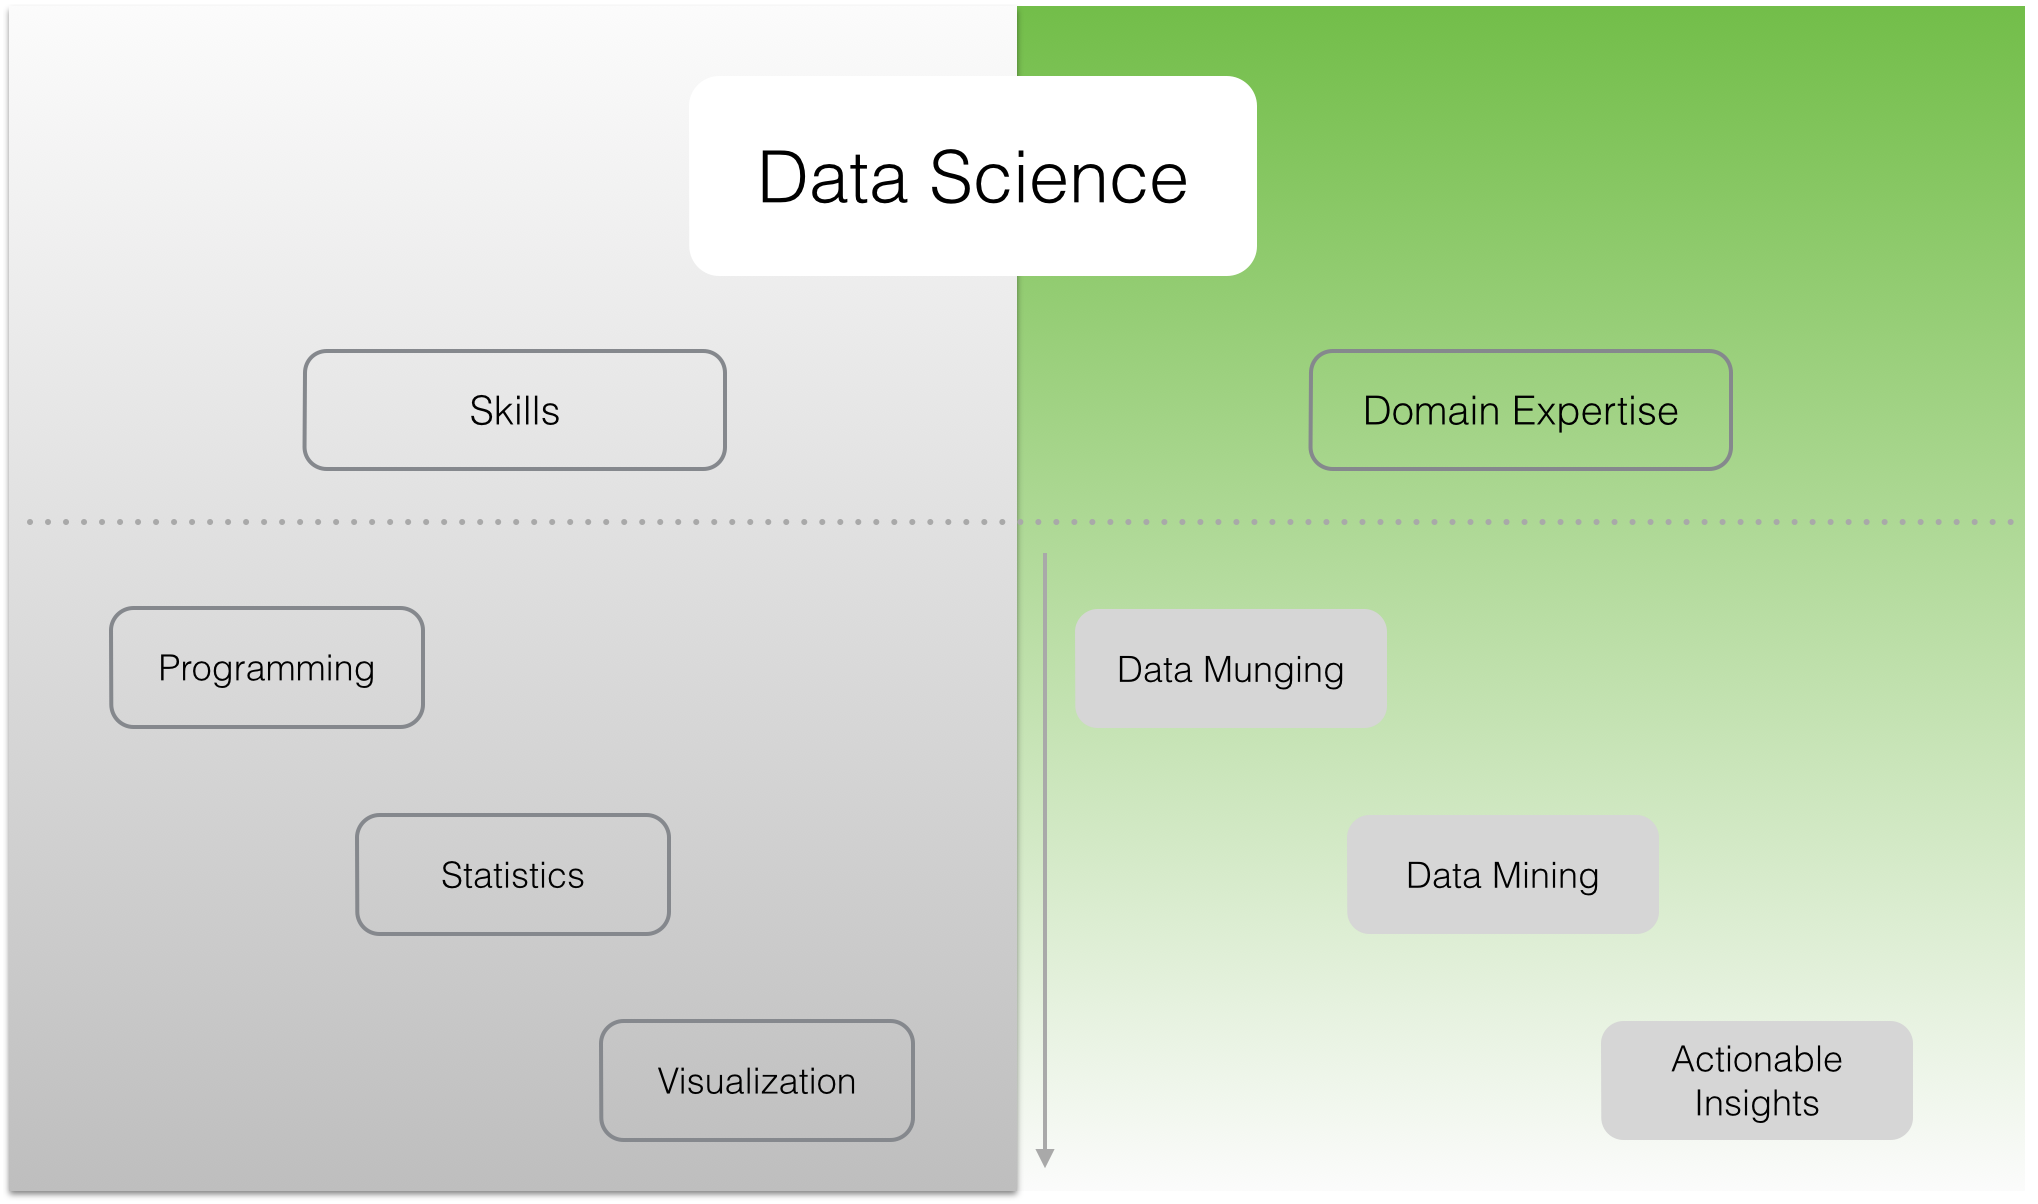
\includegraphics[width=300pt]{../graphs/data_science_structure}
      \end{center}
    \end{frame}

  \subsection{Skills and Domain Expertise}
  
    \begin{frame}{Domain expertise of a data scientist}
      \begin{center}
        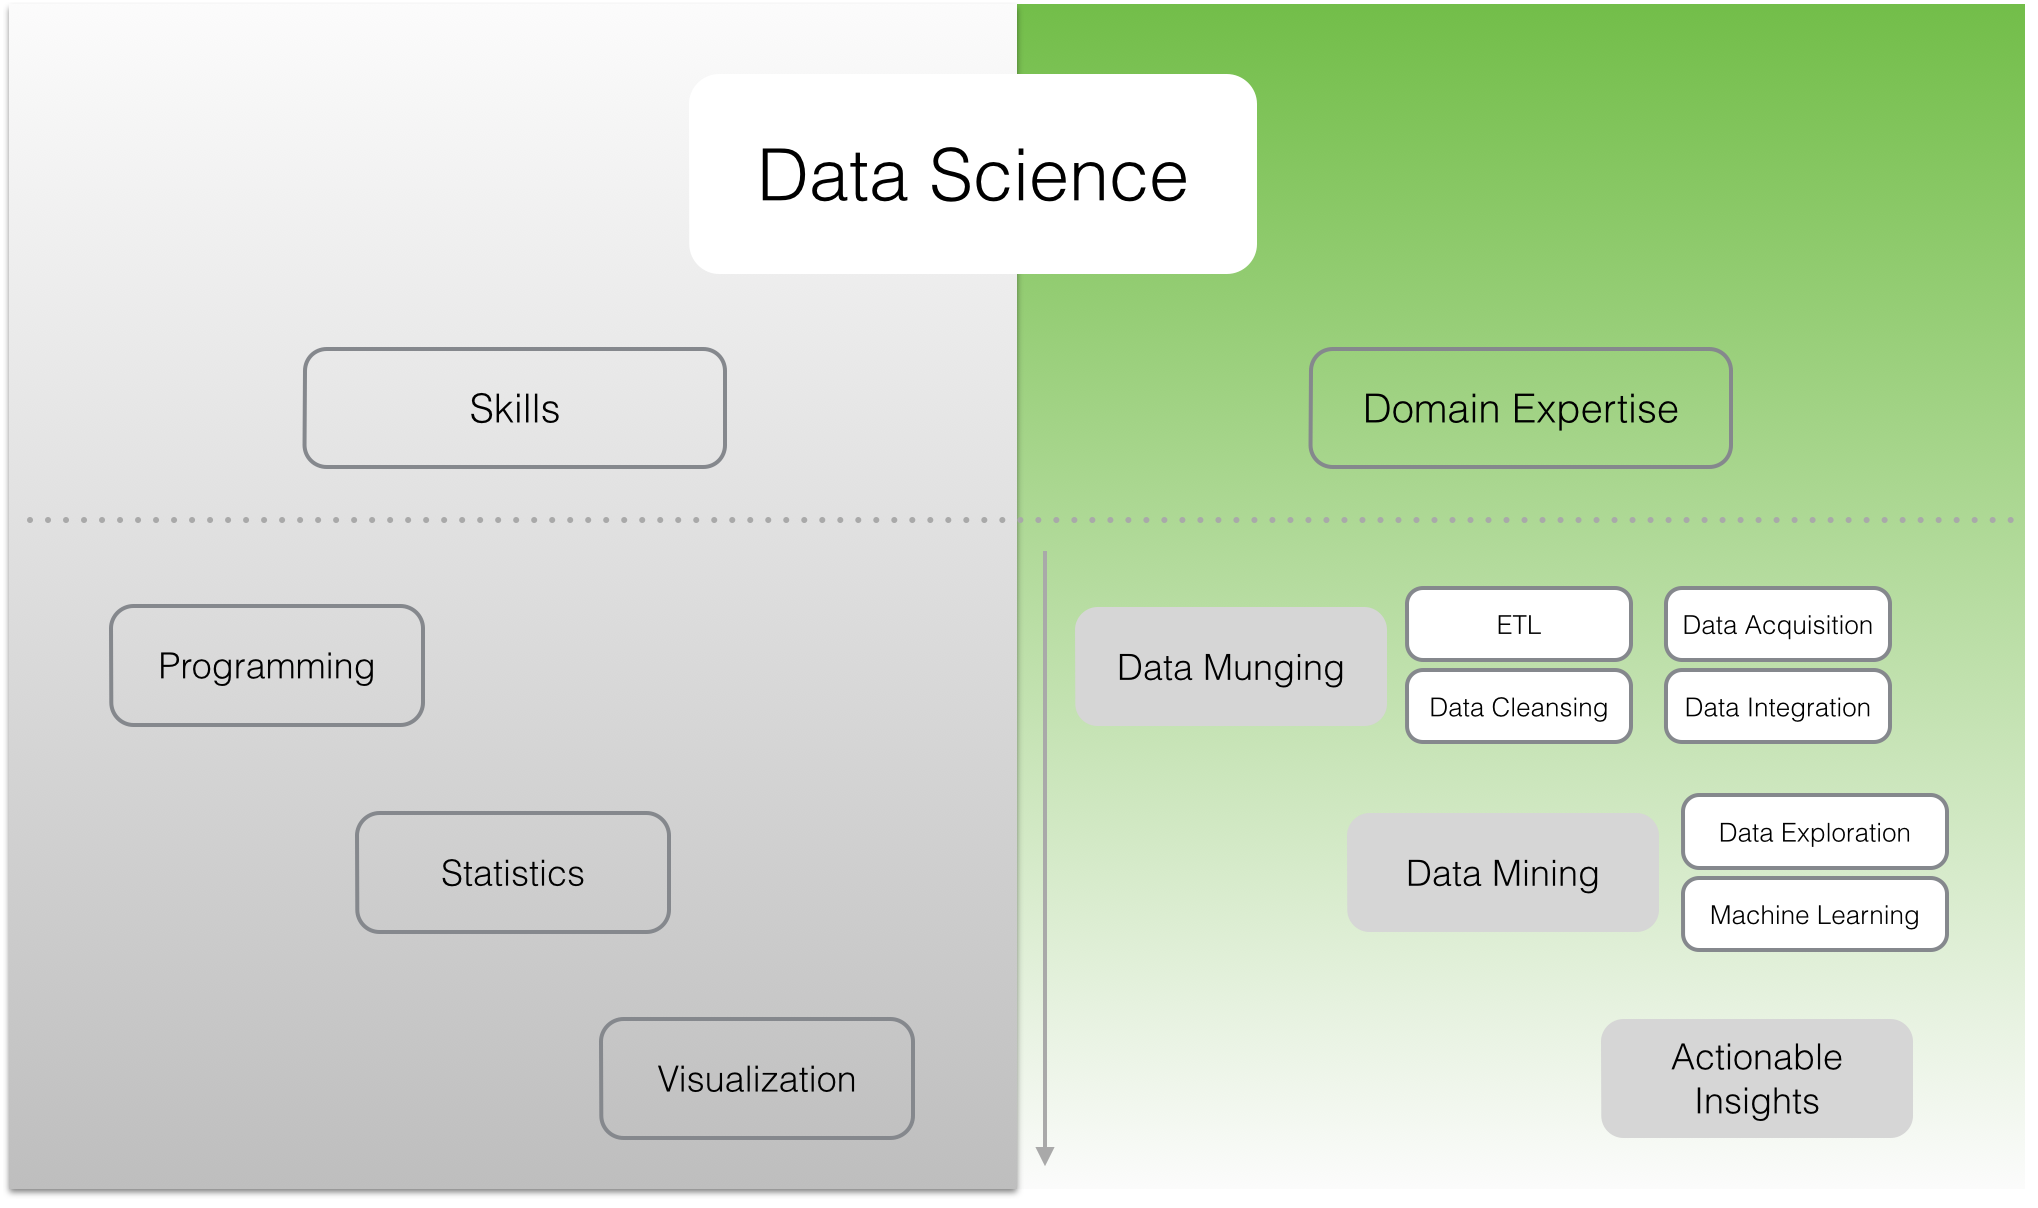
\includegraphics[width=300pt]{../graphs/data_science_domain}
      \end{center}
    \end{frame}

    \begin{frame}{Skills of a data scientist}
      \begin{center}
        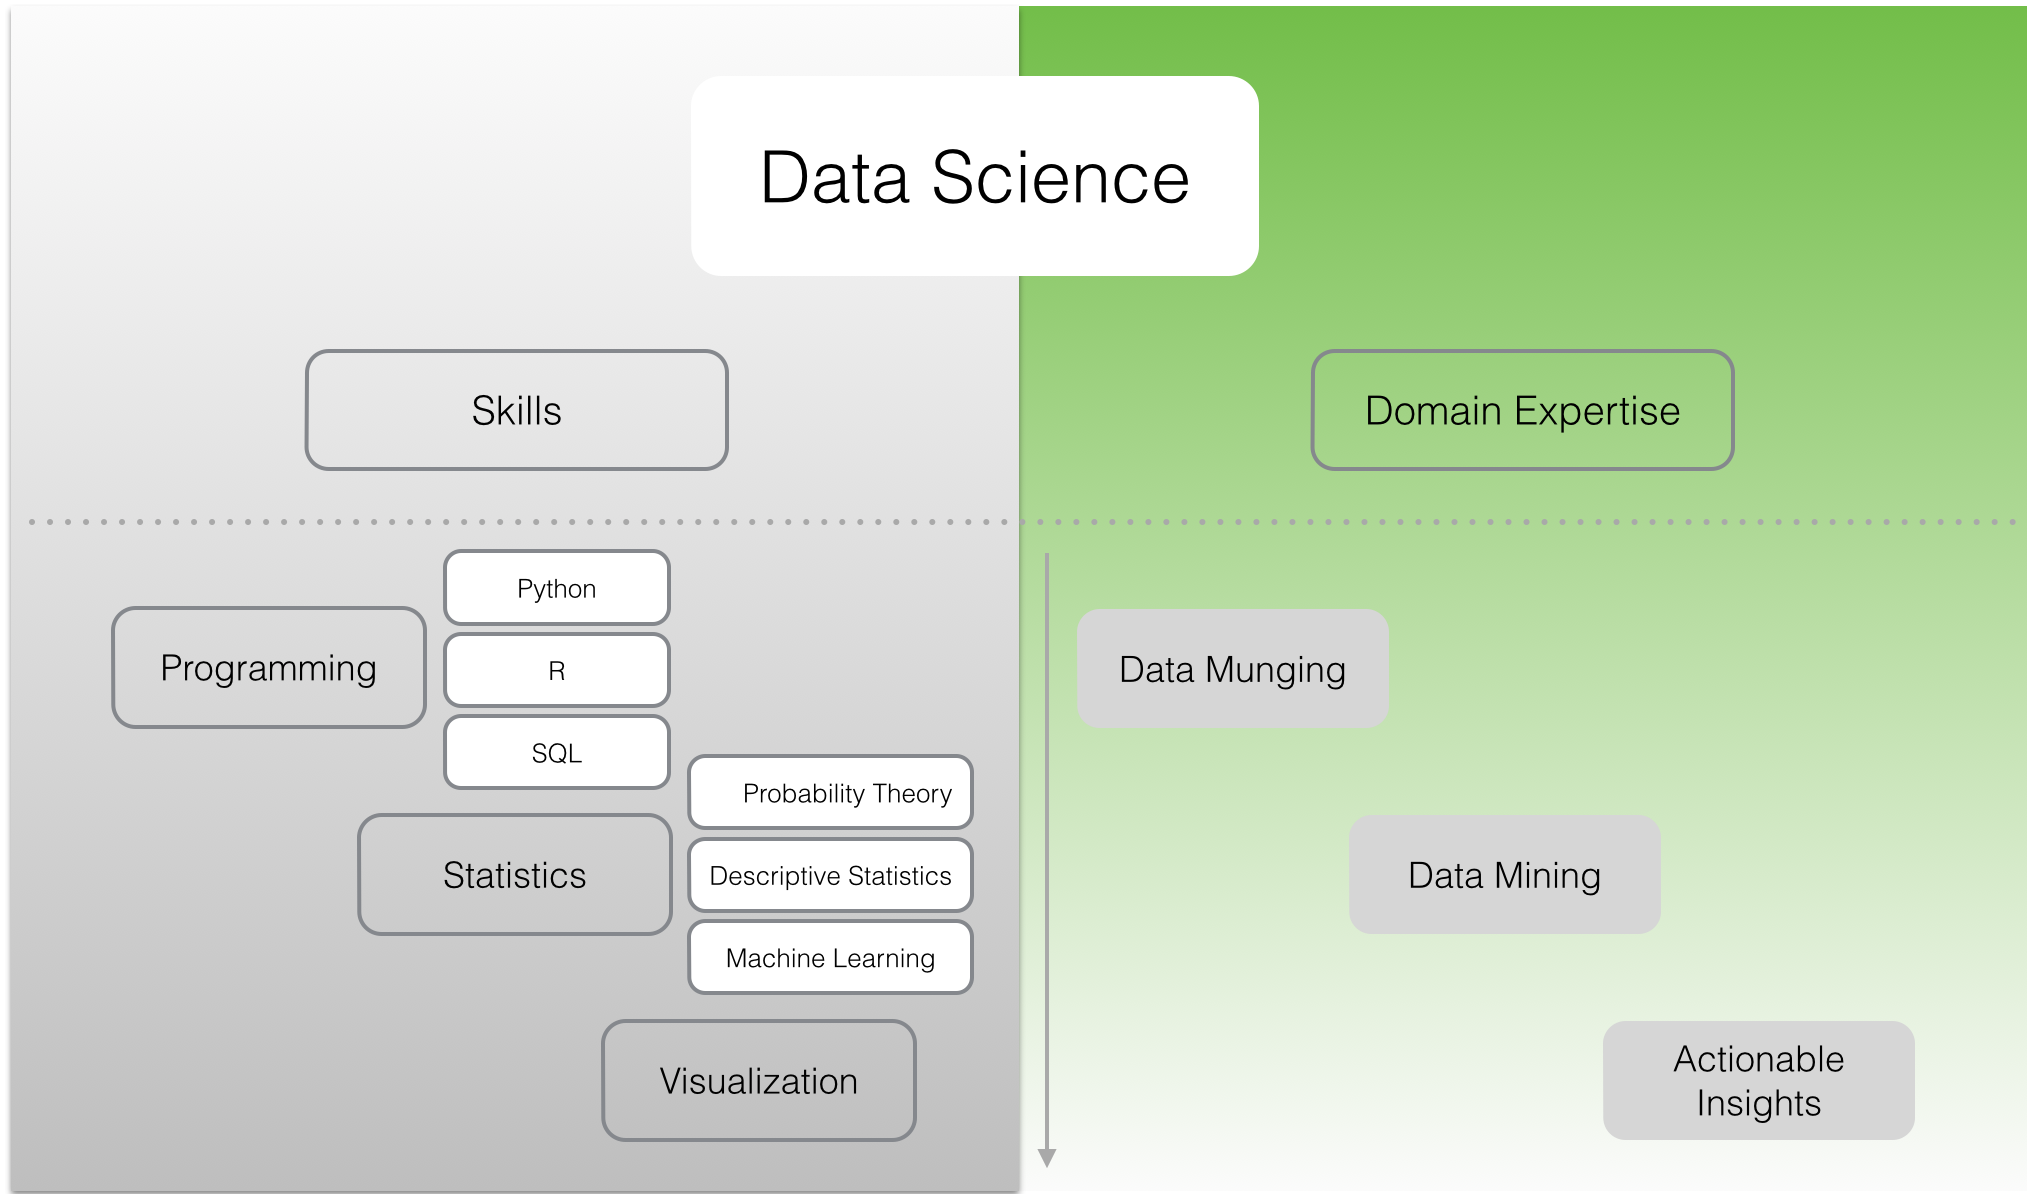
\includegraphics[width=300pt]{../graphs/data_science_skills}
      \end{center}
    \end{frame}

    \begin{frame}{Doing data science}
      \begin{center}
        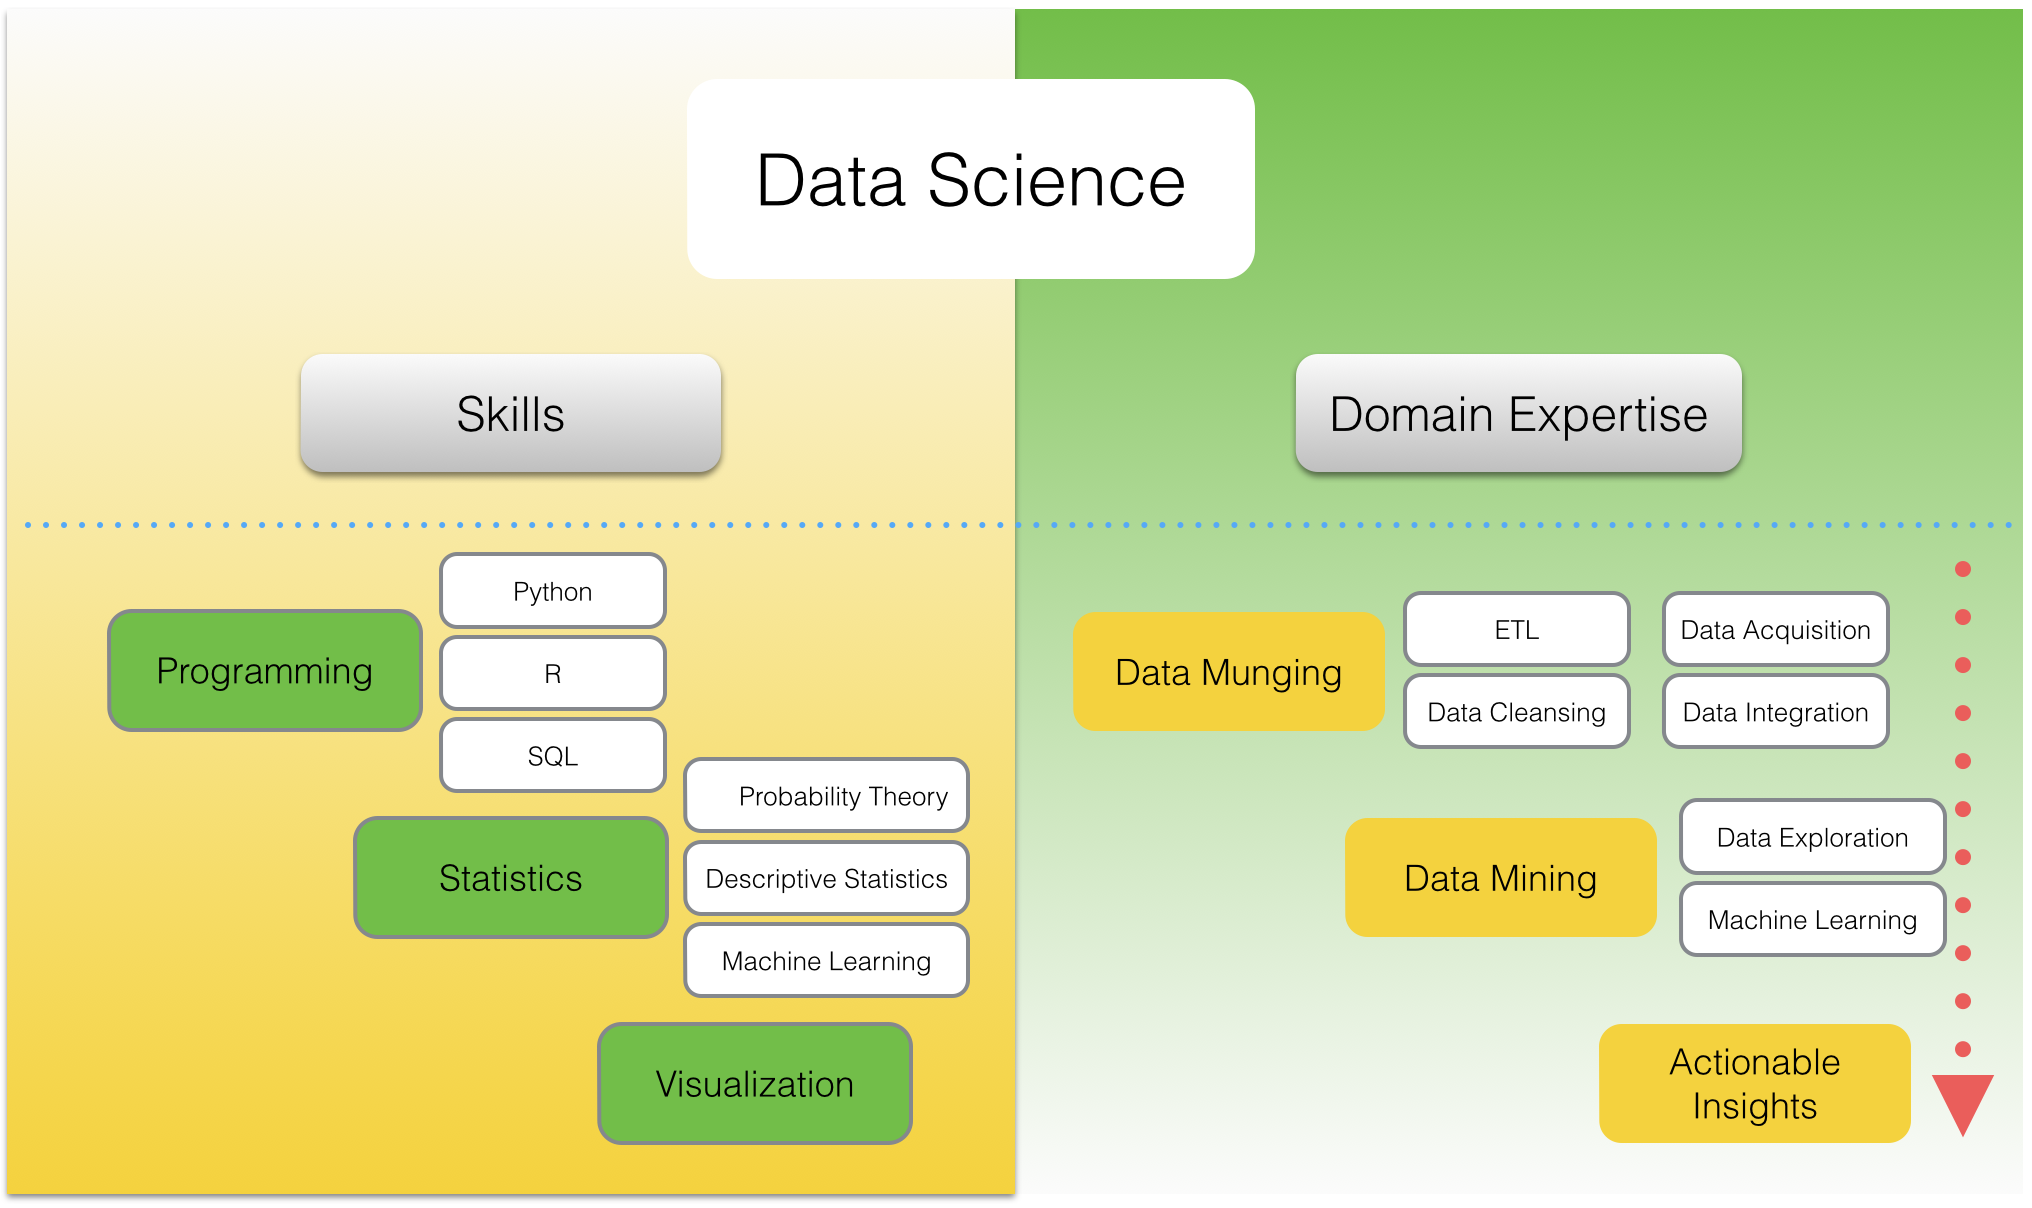
\includegraphics[width=300pt]{../graphs/data_science_skills_domain}
      \end{center}
    \end{frame}

\section{Data Science in Action}

  \subsection{Churn Model: Business Understanding}

      \begin{frame}{The quest}
        \setbeamercovered{transparent}
        \begin{block}{Definition of a churned customer}
        \end{block}
        \pause
        \begin{block}{Goal}
            \begin{itemize}
              \item To predict which customers will churn.
            \end{itemize}
        \end{block}
        \pause
        \begin{block}{Data sets}
          \begin{itemize}
            \item Customer renew data.
            \item Customer support data.
            \item Customer account and demographic data.
            \item Customer usage data.
          \end{itemize}
        \end{block}
      \end{frame}

    \begin{frame}{Customer renewal data}
        \begin{columns}[c]
          \column{.5\textwidth}
          \begin{block}{Raw data}
            \begin{center}
              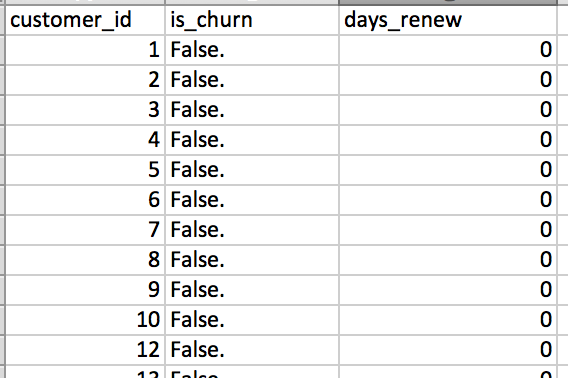
\includegraphics[height=100pt]{../graphs/dataset_customer_renew}
            \end{center}
          \end{block}
          \column{.5\textwidth}
          \begin{block}{Renewal Schedule}
            \begin{center}
              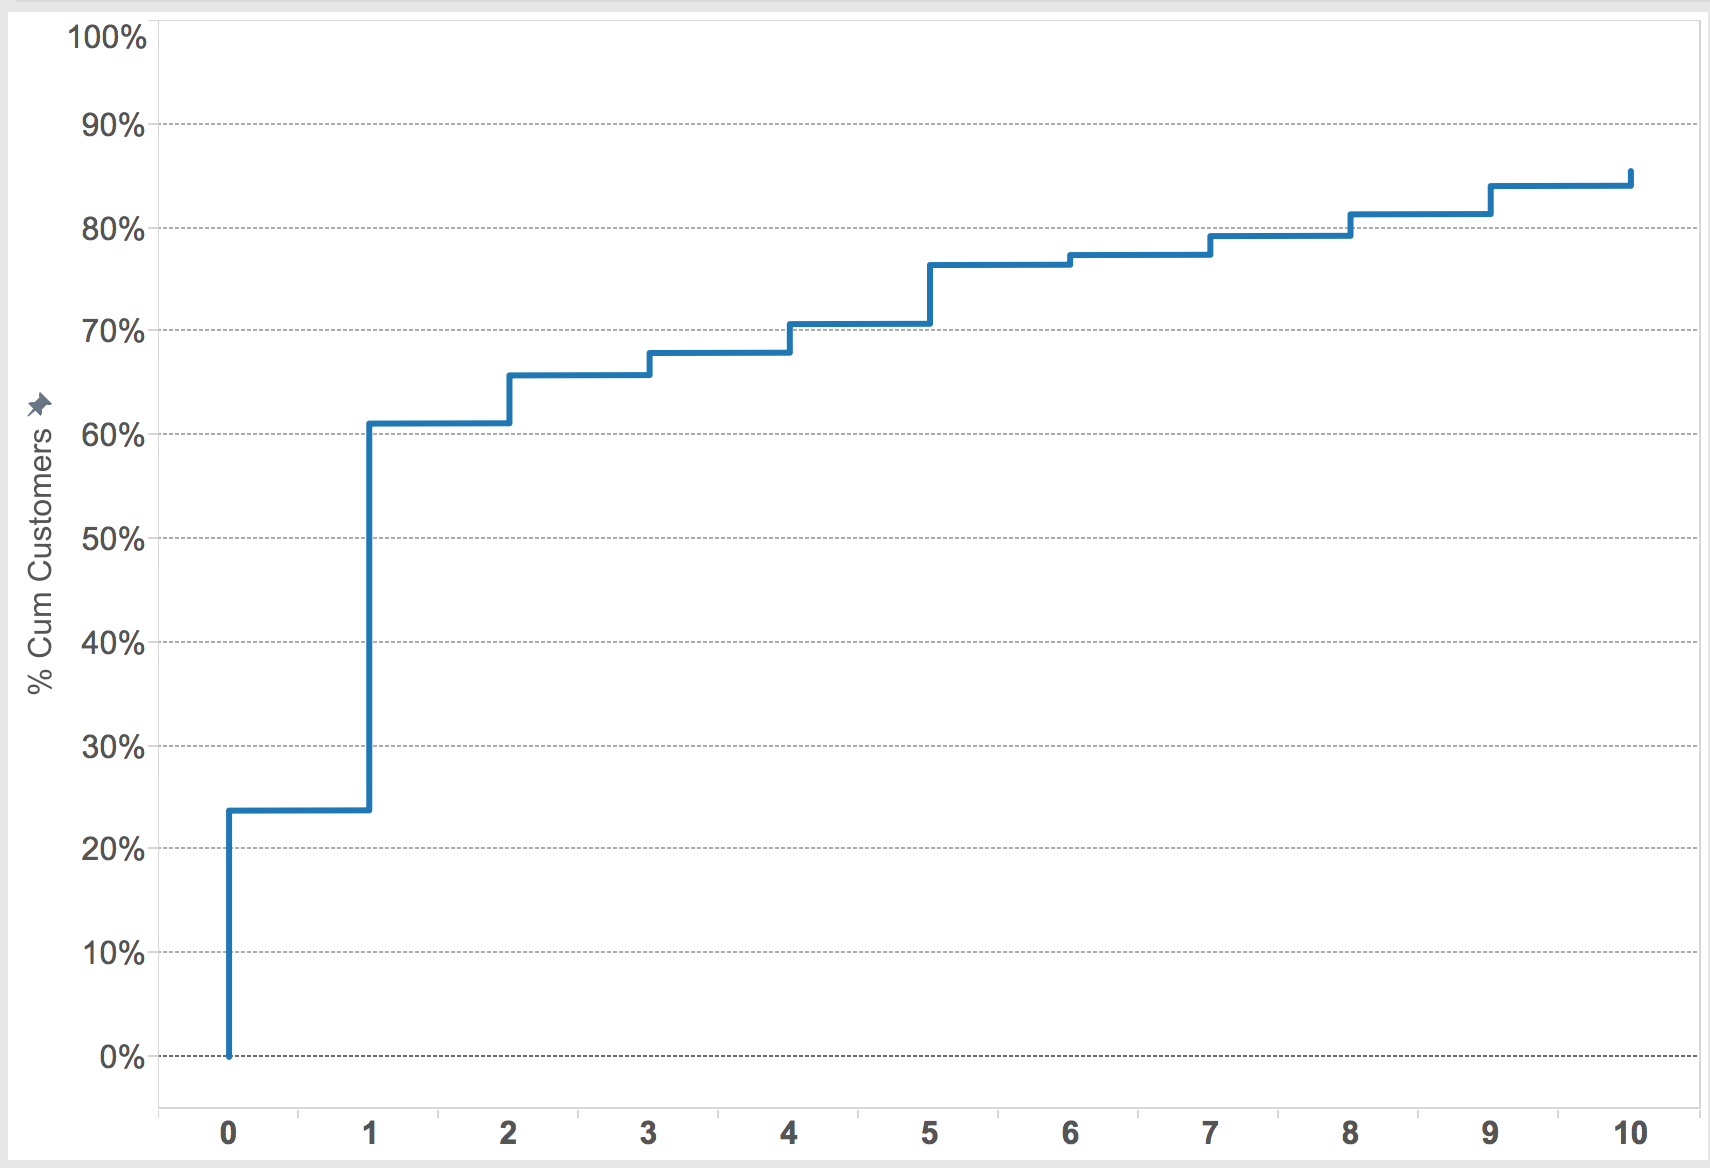
\includegraphics[height=100pt]{../graphs/dataset_renewal_schedule}
            \end{center}
          \end{block}
        \end{columns}
    \end{frame}

    \begin{frame}{Customer service call data}
        \begin{columns}[c]
          \column{.5\textwidth}
          \begin{block}{Raw data}
            \begin{center}
              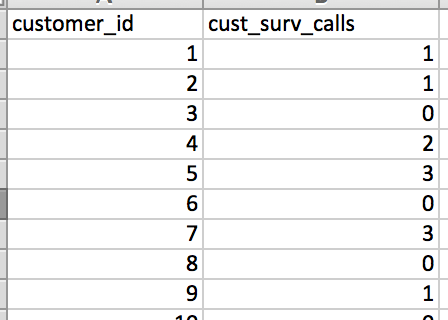
\includegraphics[height=100pt]{../graphs/dataset_customer_support}
            \end{center}
          \end{block}
          \column{.5\textwidth}
          \begin{block}{Cumulative distribution}
            \begin{center}
              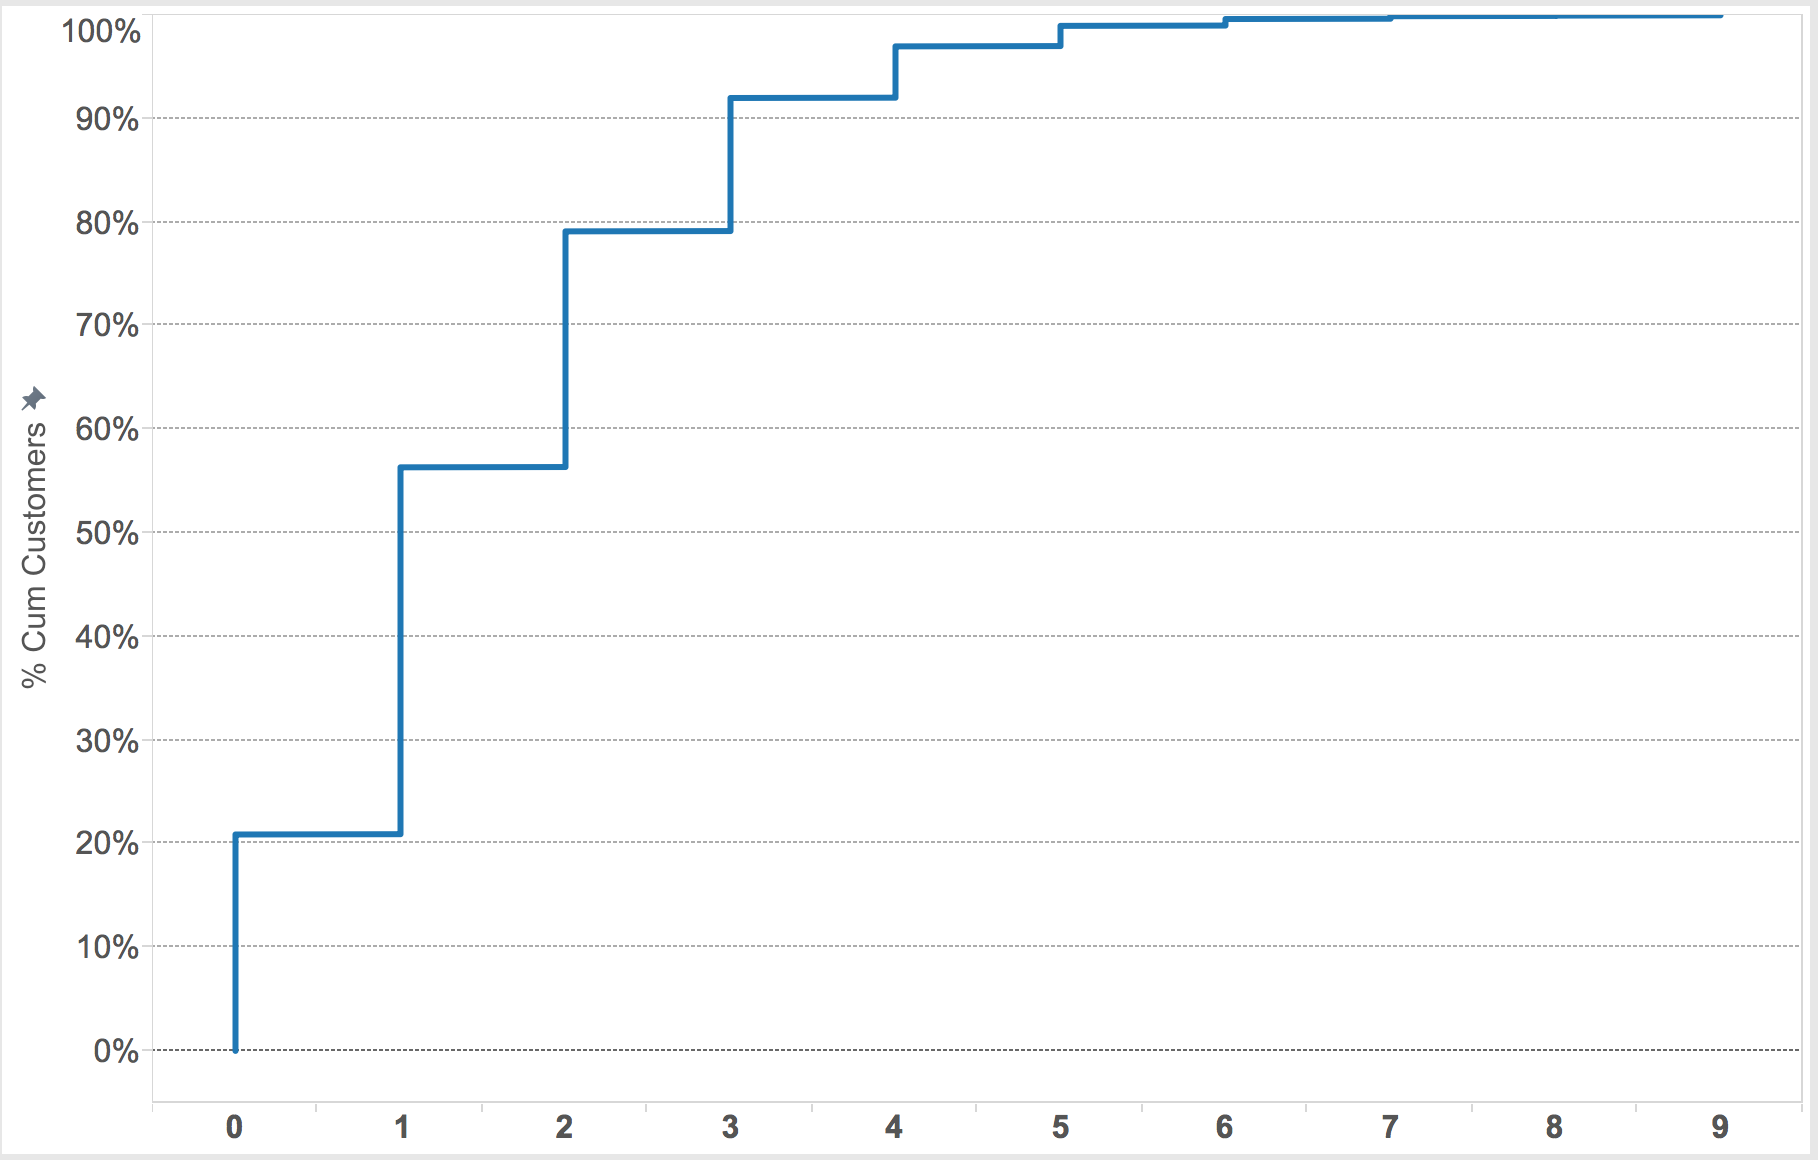
\includegraphics[height=100pt]{../graphs/dataset_cust_call_chart}
            \end{center}
          \end{block}
        \end{columns}
    \end{frame}

    \begin{frame}{Customer plan type and demographic}
        \begin{center}
          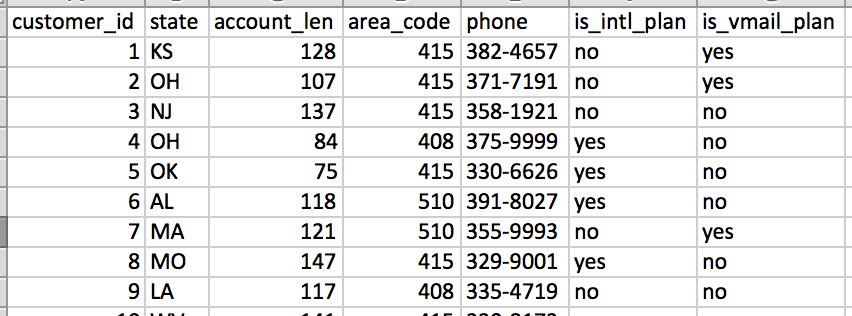
\includegraphics[height=120pt]{../graphs/dataset_customer_account}
        \end{center}
    \end{frame}

    \begin{frame}{Customer usage data}
        \begin{center}
          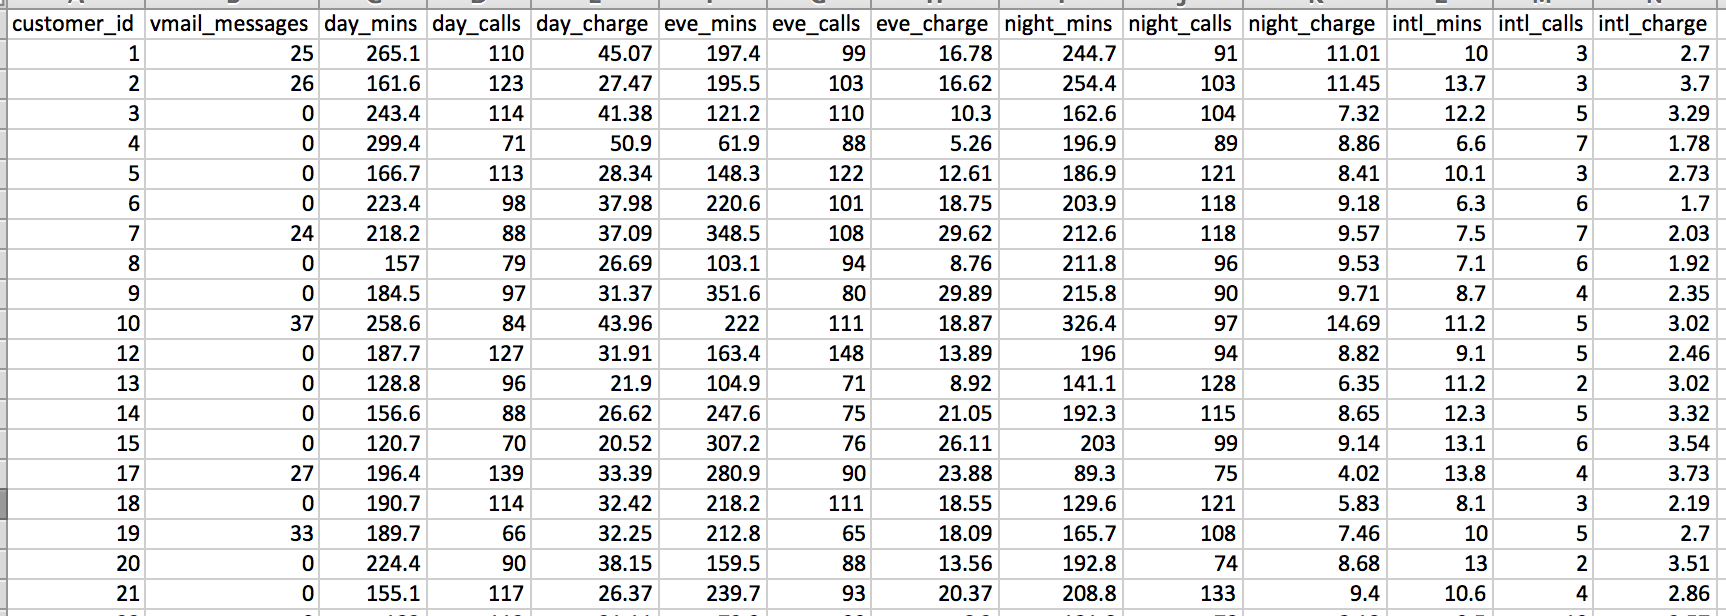
\includegraphics[height=100pt]{../graphs/dataset_customer_usage}
        \end{center}
    \end{frame}

    \begin{frame}{Churn data structure}
      \begin{center}
        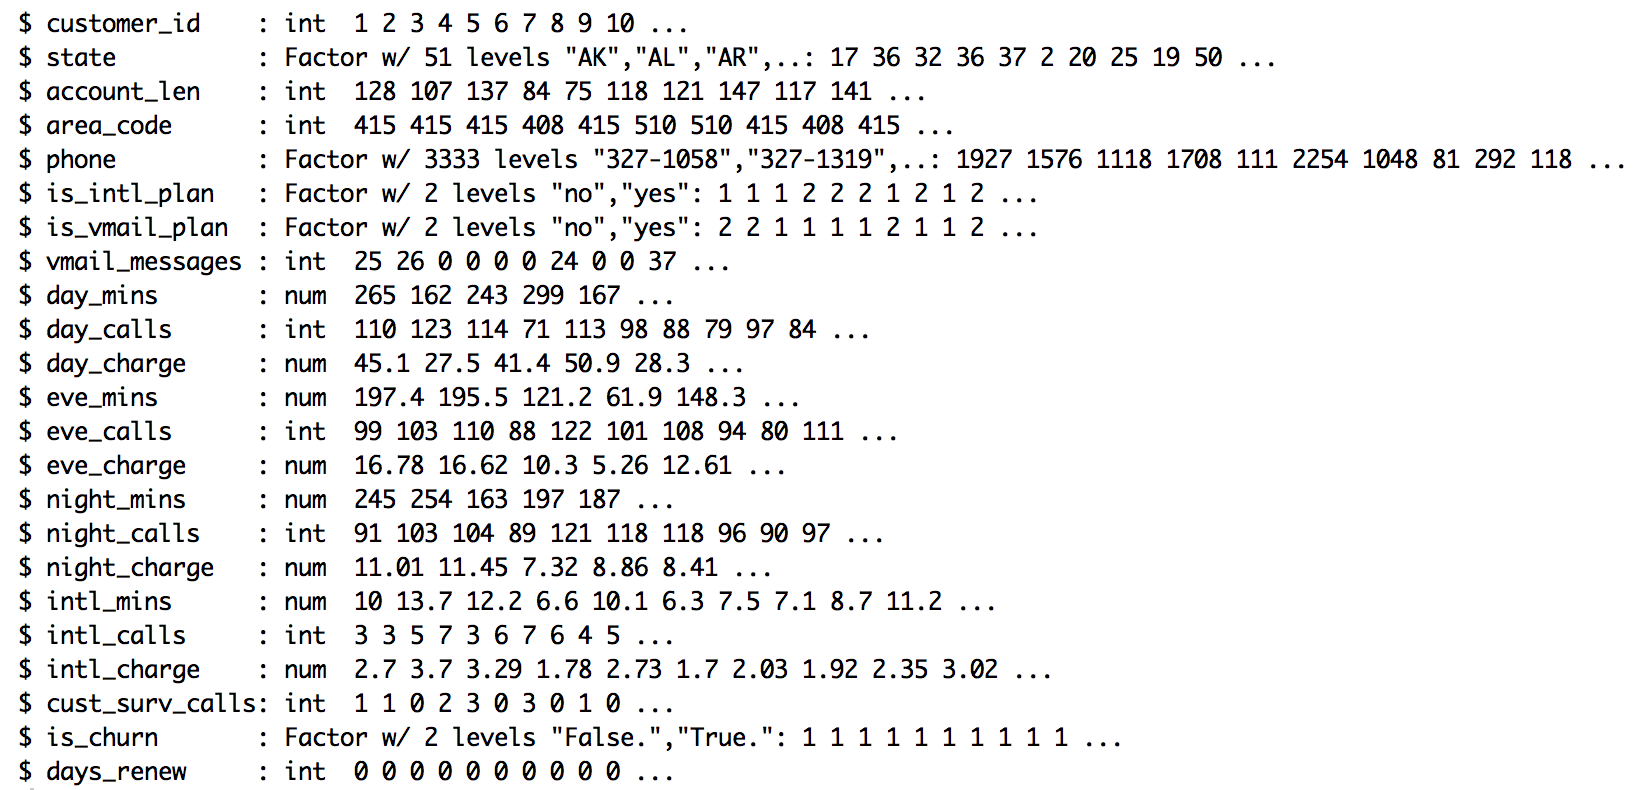
\includegraphics[height=180pt]{../graphs/dataset_churn_str}
      \end{center}
    \end{frame}

  \subsection{Churn Model: Demo in R}

    \begin{frame}{R Script}
        \begin{center}
          {\large \url{https://github.com/vieplivee/Data-Science-in-Action/blob/master/src/churn.R}}
        \end{center}
    \end{frame}
    
  \subsection{Churn Model: Top Features}
  
    \begin{frame}{Variable importance from random forest}
        \begin{center}
          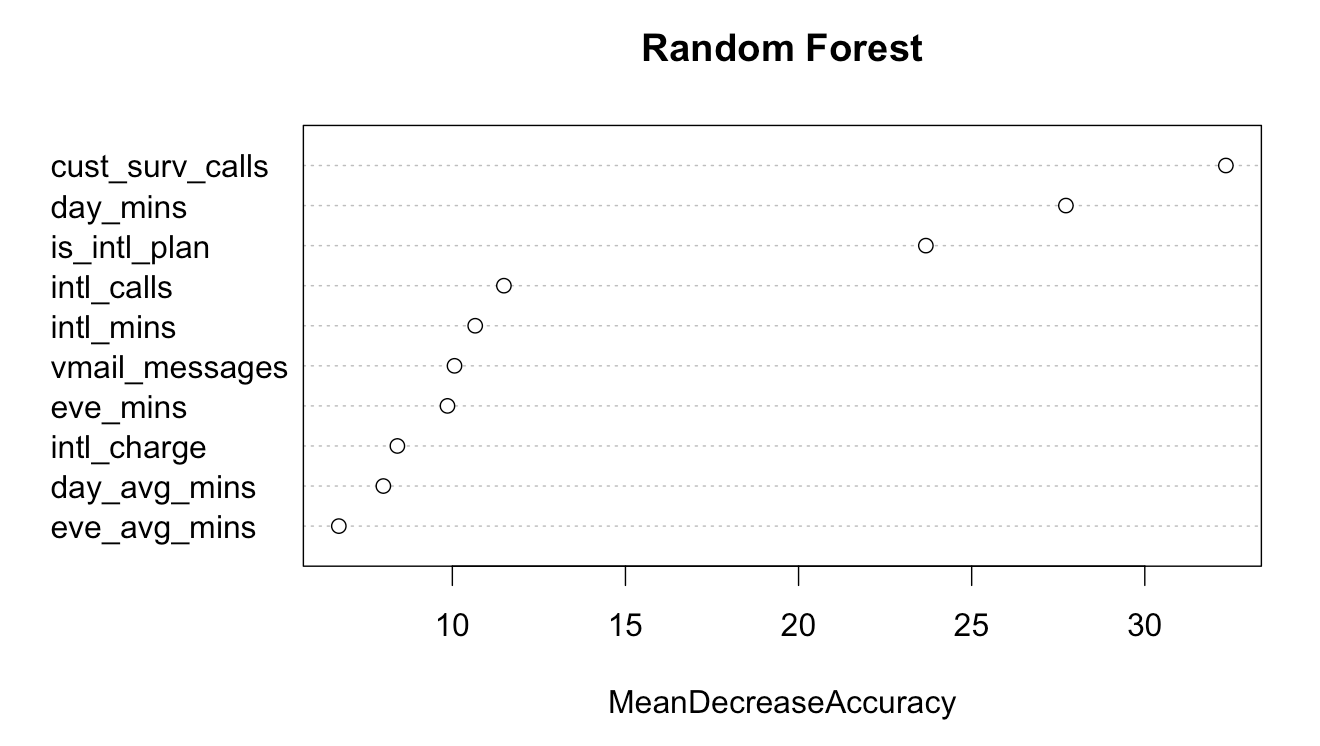
\includegraphics[width=300pt]{../graphs/rf_var_importance}
        \end{center}
    \end{frame}

    \begin{frame}{Top feature - customer service calls}
      \begin{center}
        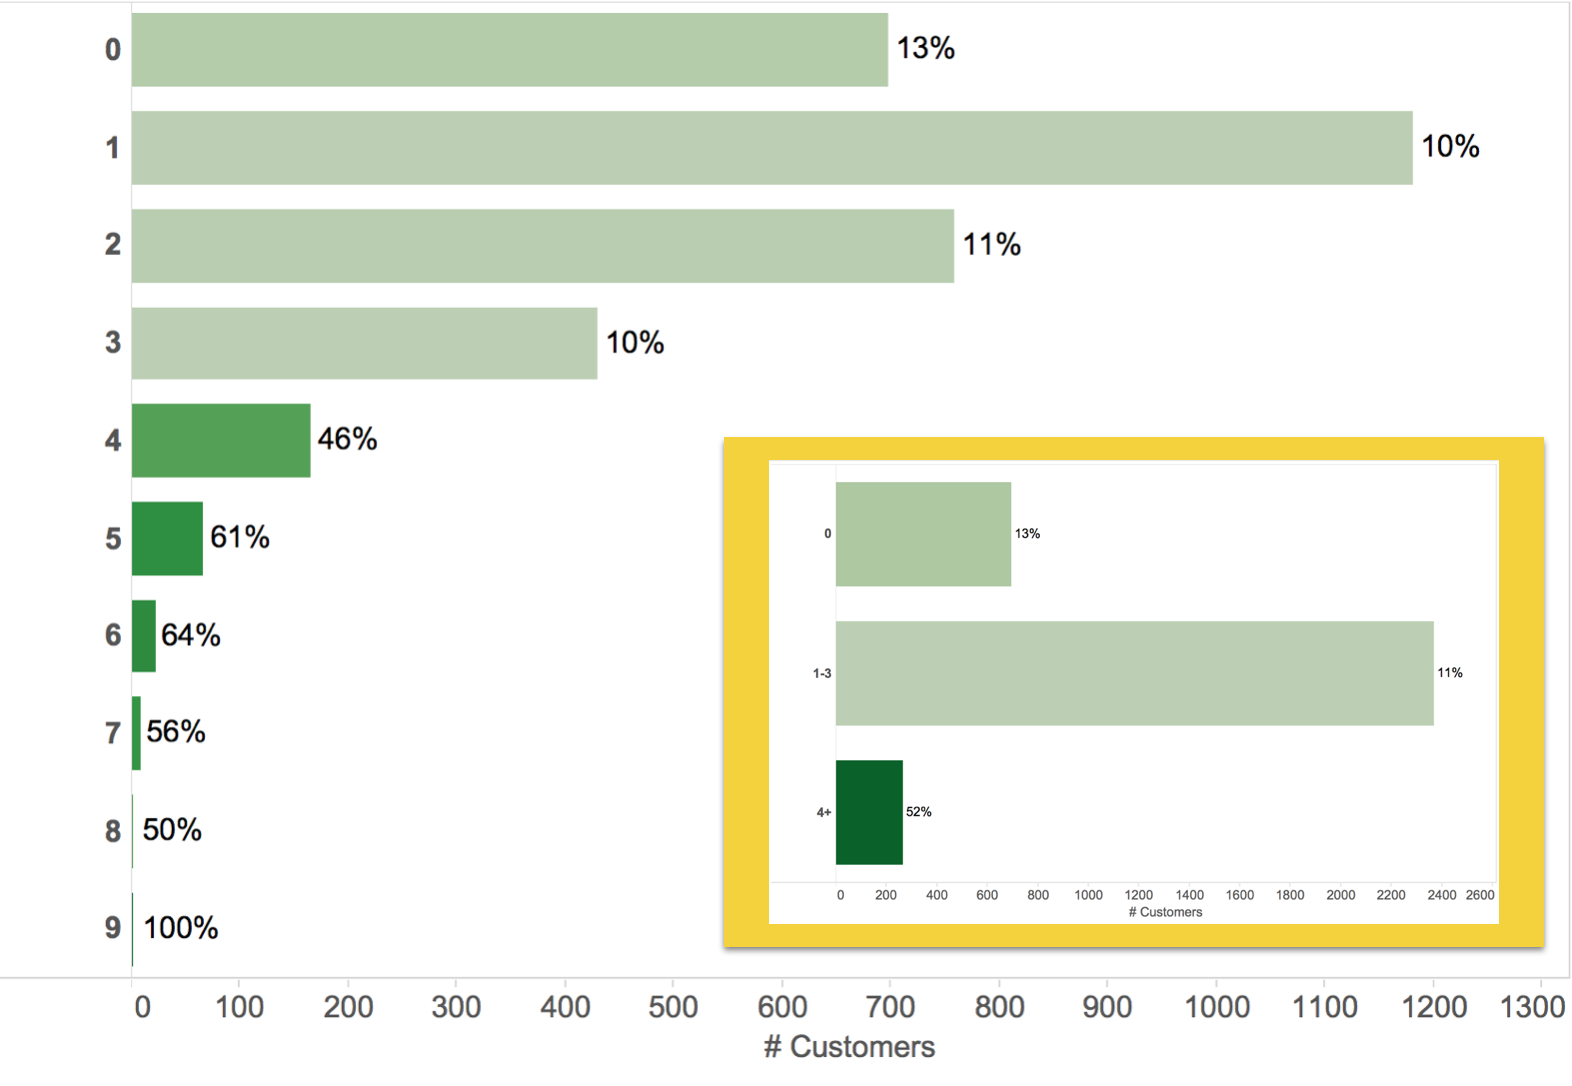
\includegraphics[width=280pt]{../graphs/top_var_cust_surv_with_group}
      \end{center}
    \end{frame}

    \begin{frame}{Top feature - customer day time minutes}
      \begin{center}
        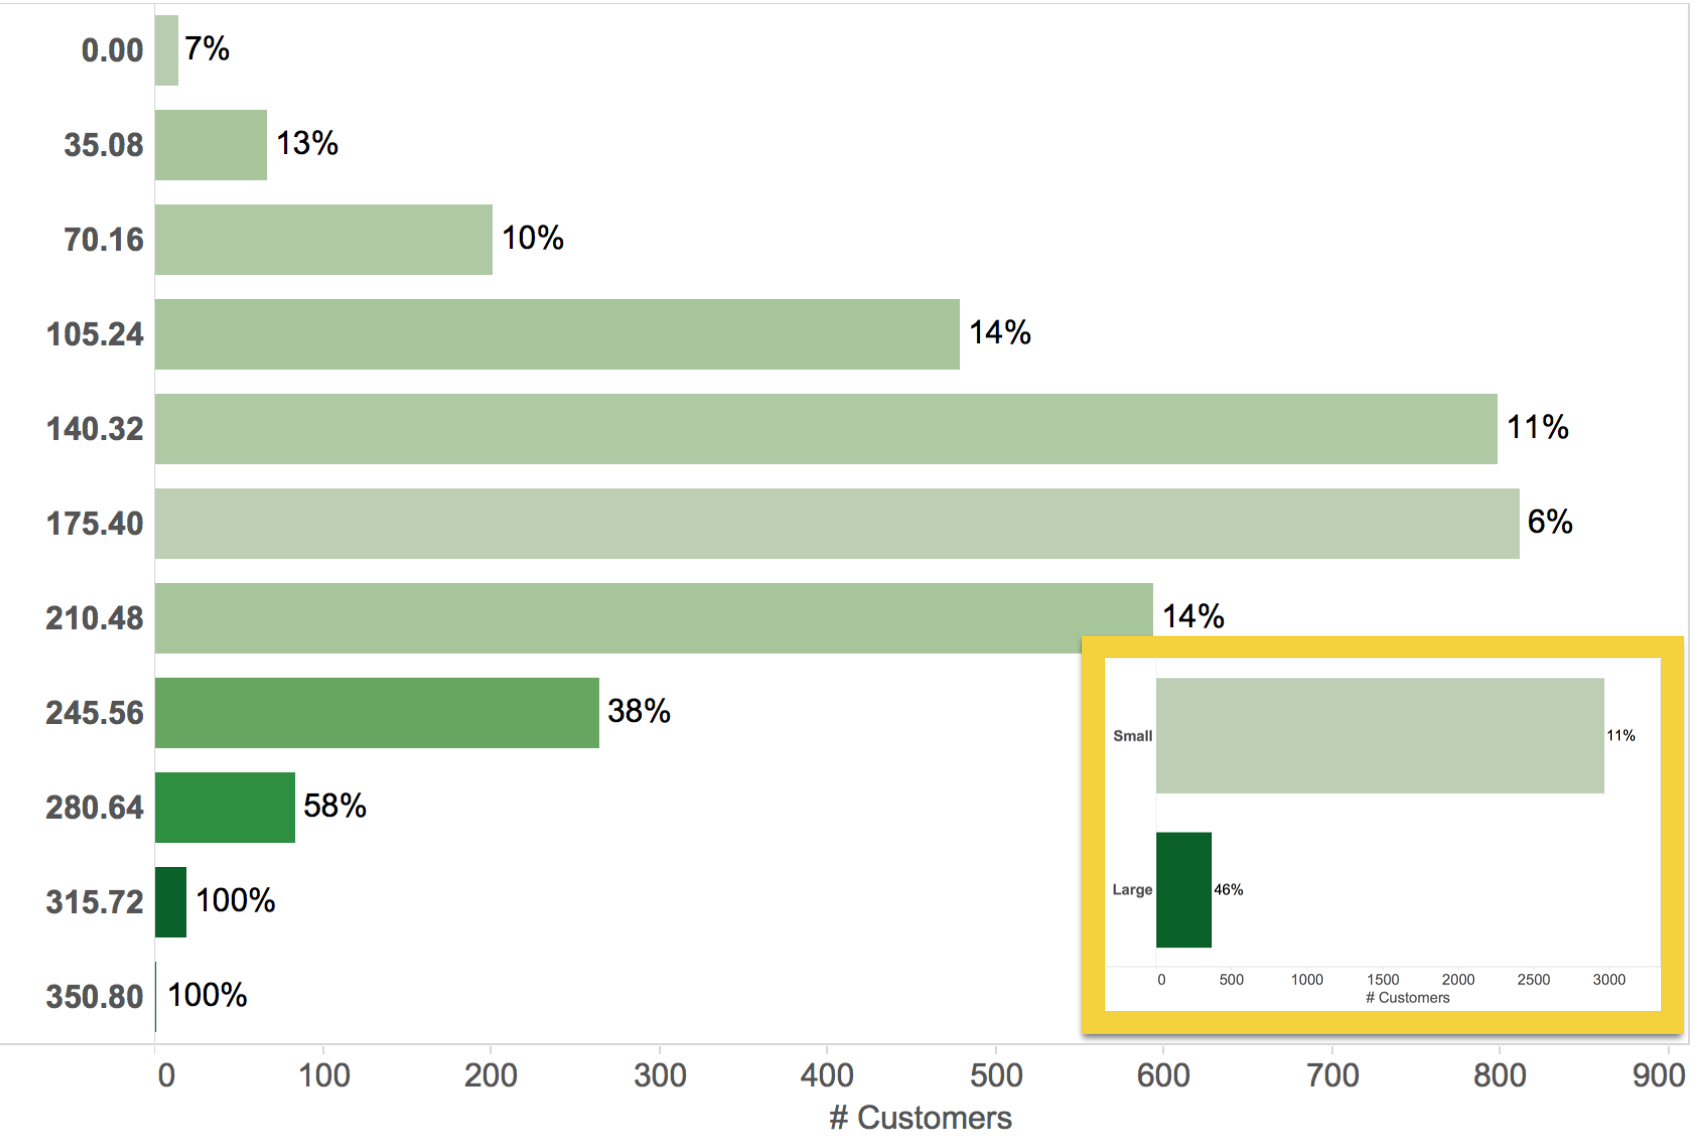
\includegraphics[width=280pt]{../graphs/top_var_day_mins_with_group}
      \end{center}
    \end{frame}

    \begin{frame}{Top feature - international plan and international calls}
      \begin{center}
        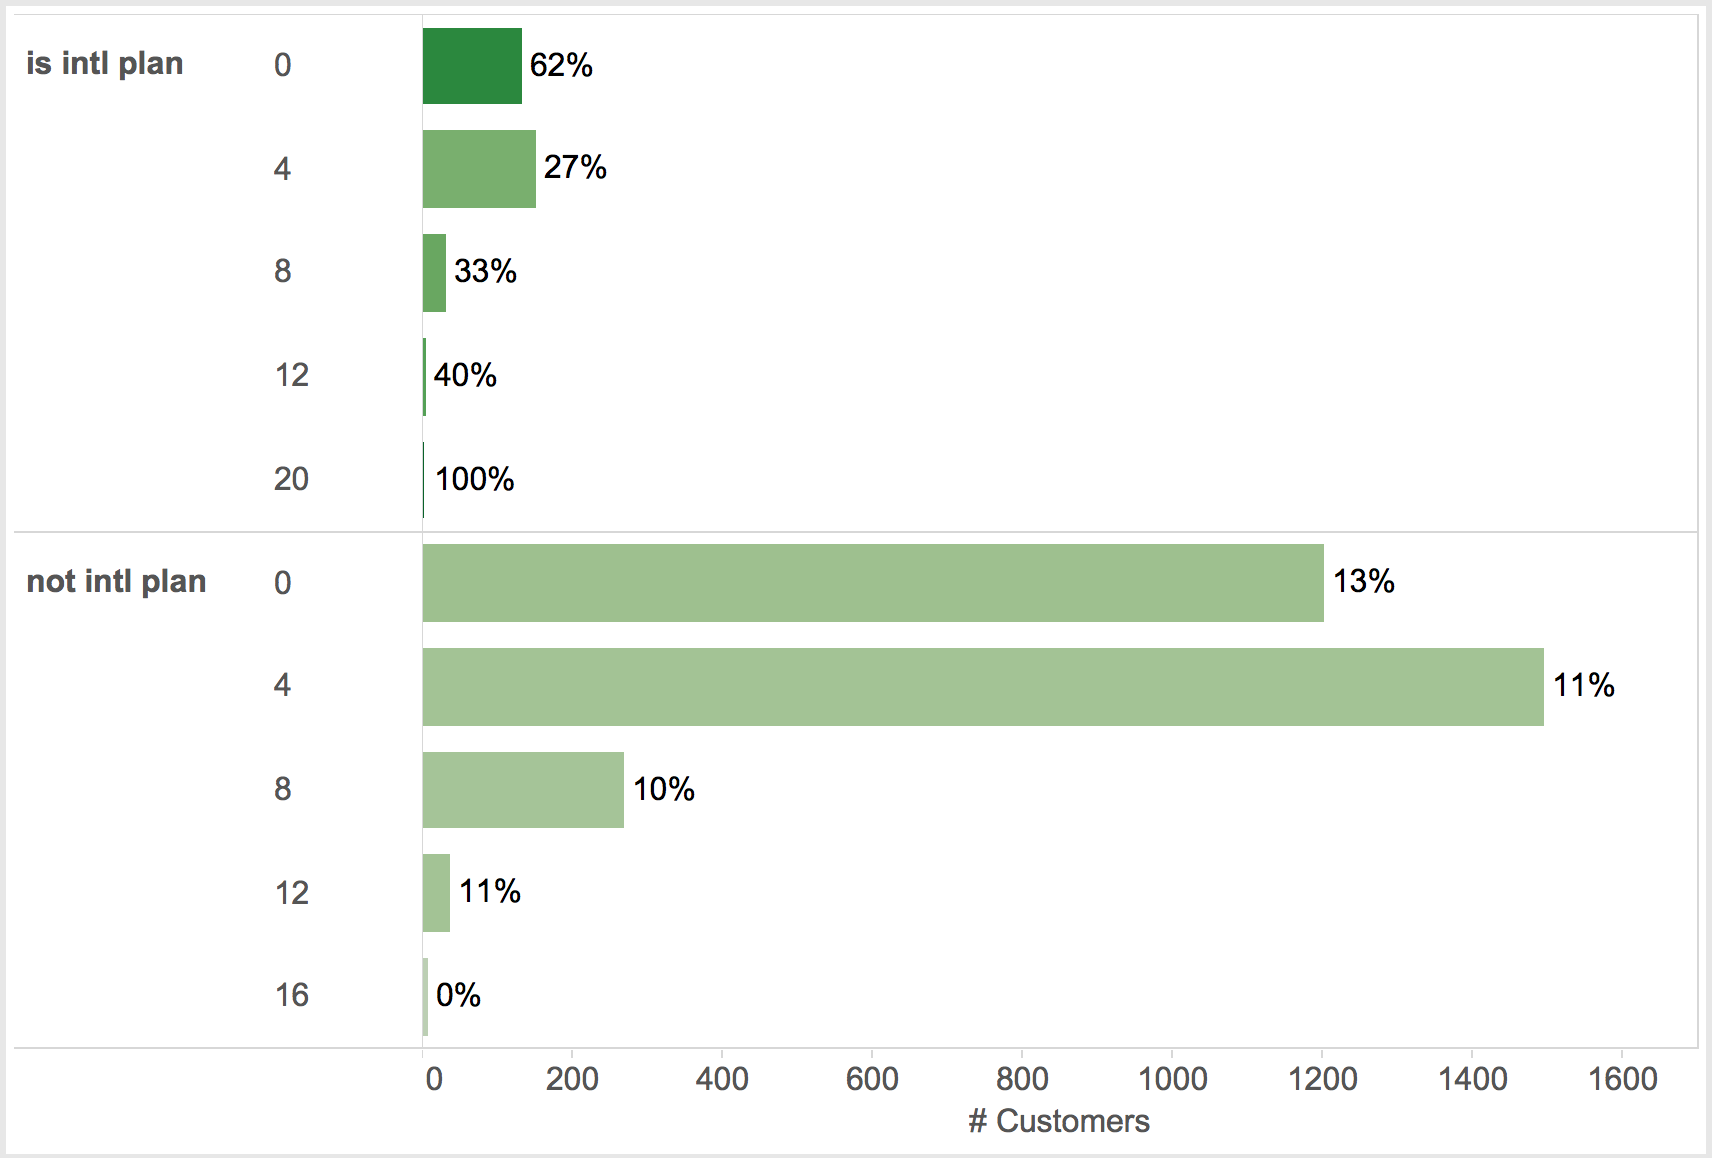
\includegraphics[width=280pt]{../graphs/top_var_intl_plan_calls}
      \end{center}
    \end{frame}

  \subsection{Churn Model: Prescriptive Analysis}

    \begin{frame}{Churn analysis}
      \begin{center}
        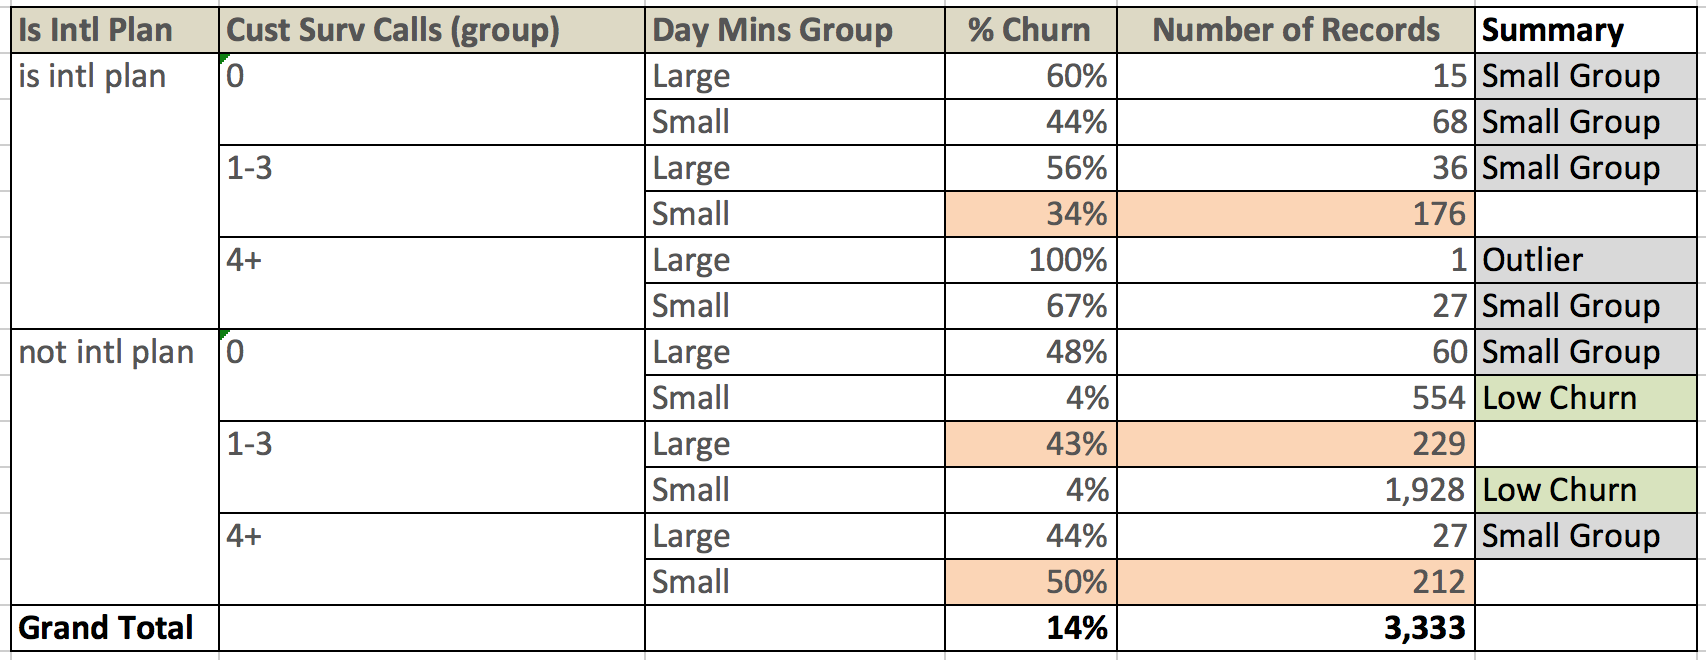
\includegraphics[height=120pt]{../graphs/churn_analysis}
      \end{center}
    \end{frame}

    \begin{frame}{Churn analysis}
      \begin{center}
        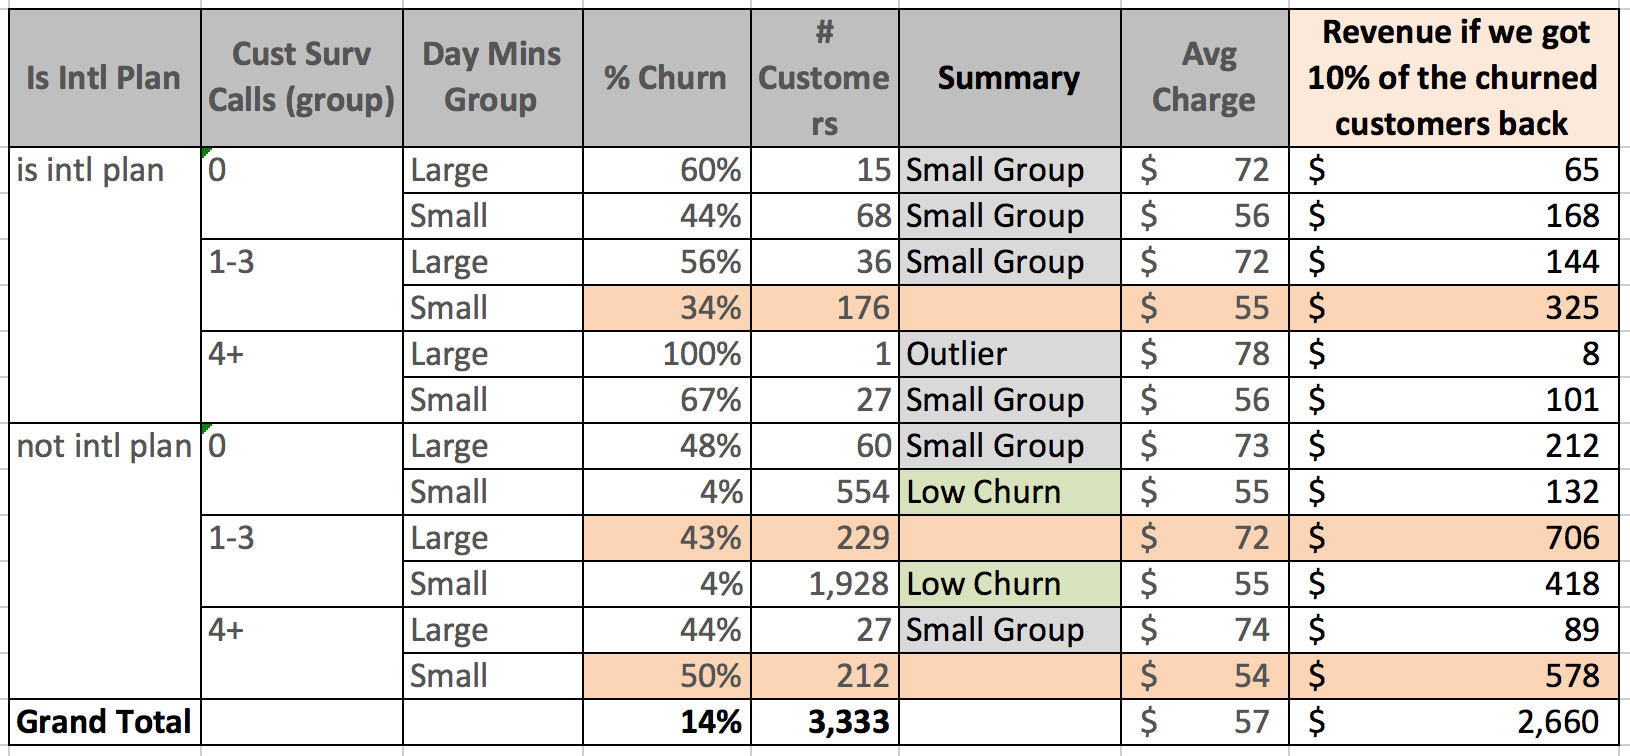
\includegraphics[height=150pt]{../graphs/churn_analysis_revenue}
      \end{center}
    \end{frame}

  \subsection{Email Analysis}

    \begin{frame}{When to send an email}
      \begin{center}
        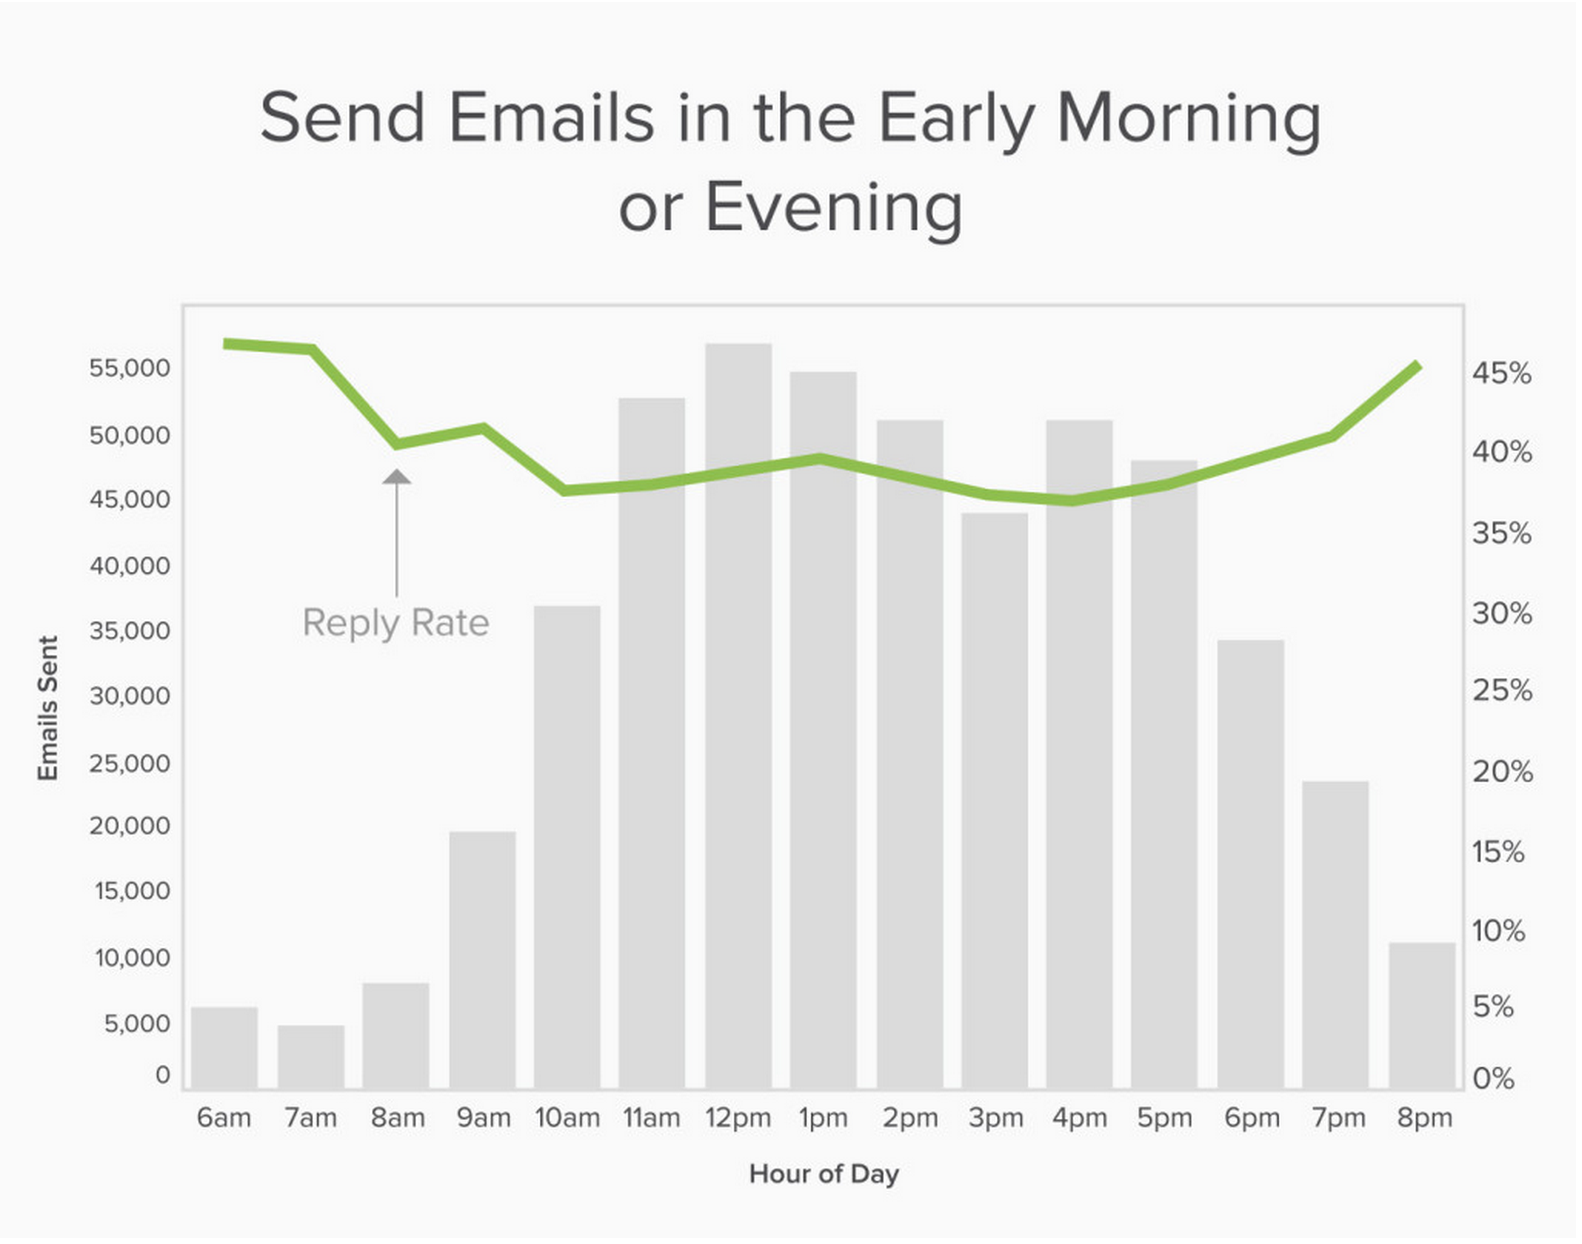
\includegraphics[height=180pt]{../graphs/email_analysis_sent_hour}
      \end{center}    
      {\footnotesize Best time to send email: \url{http://goo.gl/lVdD31}}
    \end{frame}

    \begin{frame}{D3 Visualization: Subject Line Analysis}
      \begin{center}
        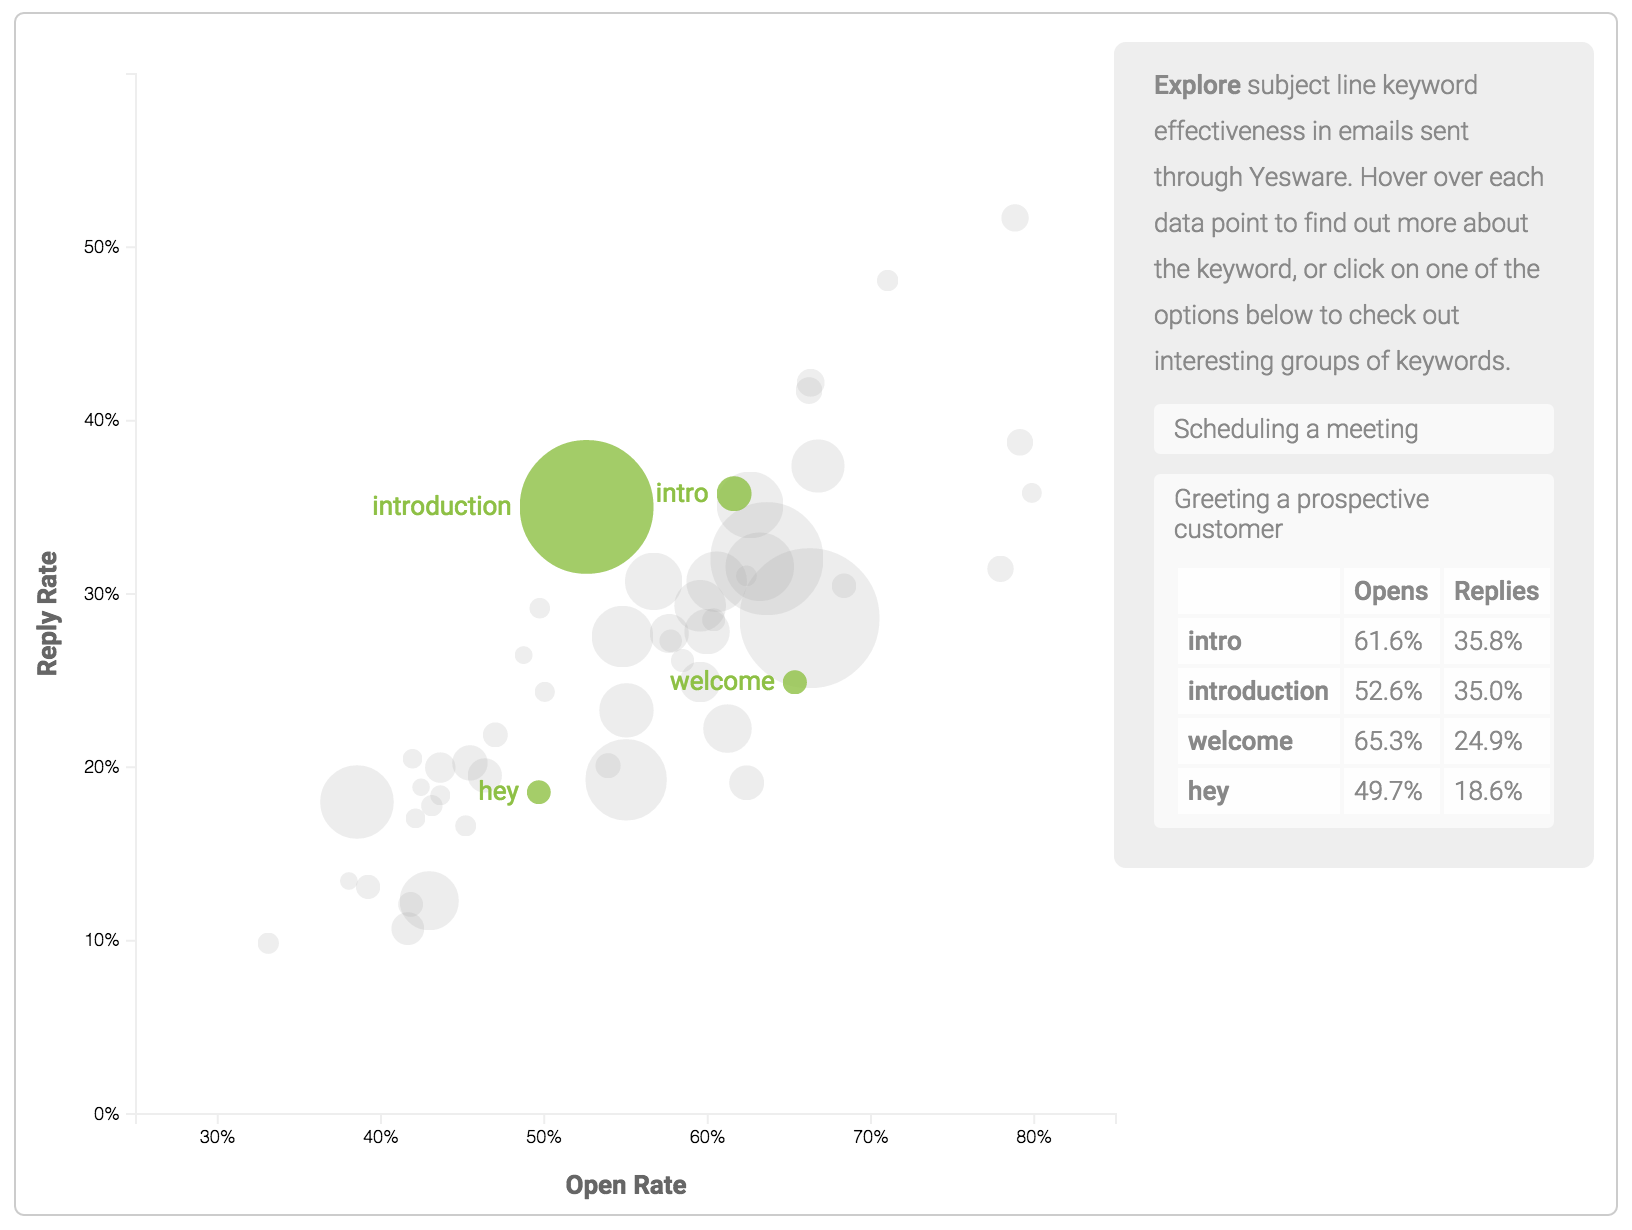
\includegraphics[height=180pt]{../graphs/email_analysis_subject_line}
      \end{center}    
      {\footnotesize Subject line key words: \url{http://goo.gl/PK9xhO}}
    \end{frame}

\section{Data Scientist Toolbox}

  \subsection{Data Scientist Toolbox}
  
    \begin{frame}{From academia to industry}
      \begin{center}
        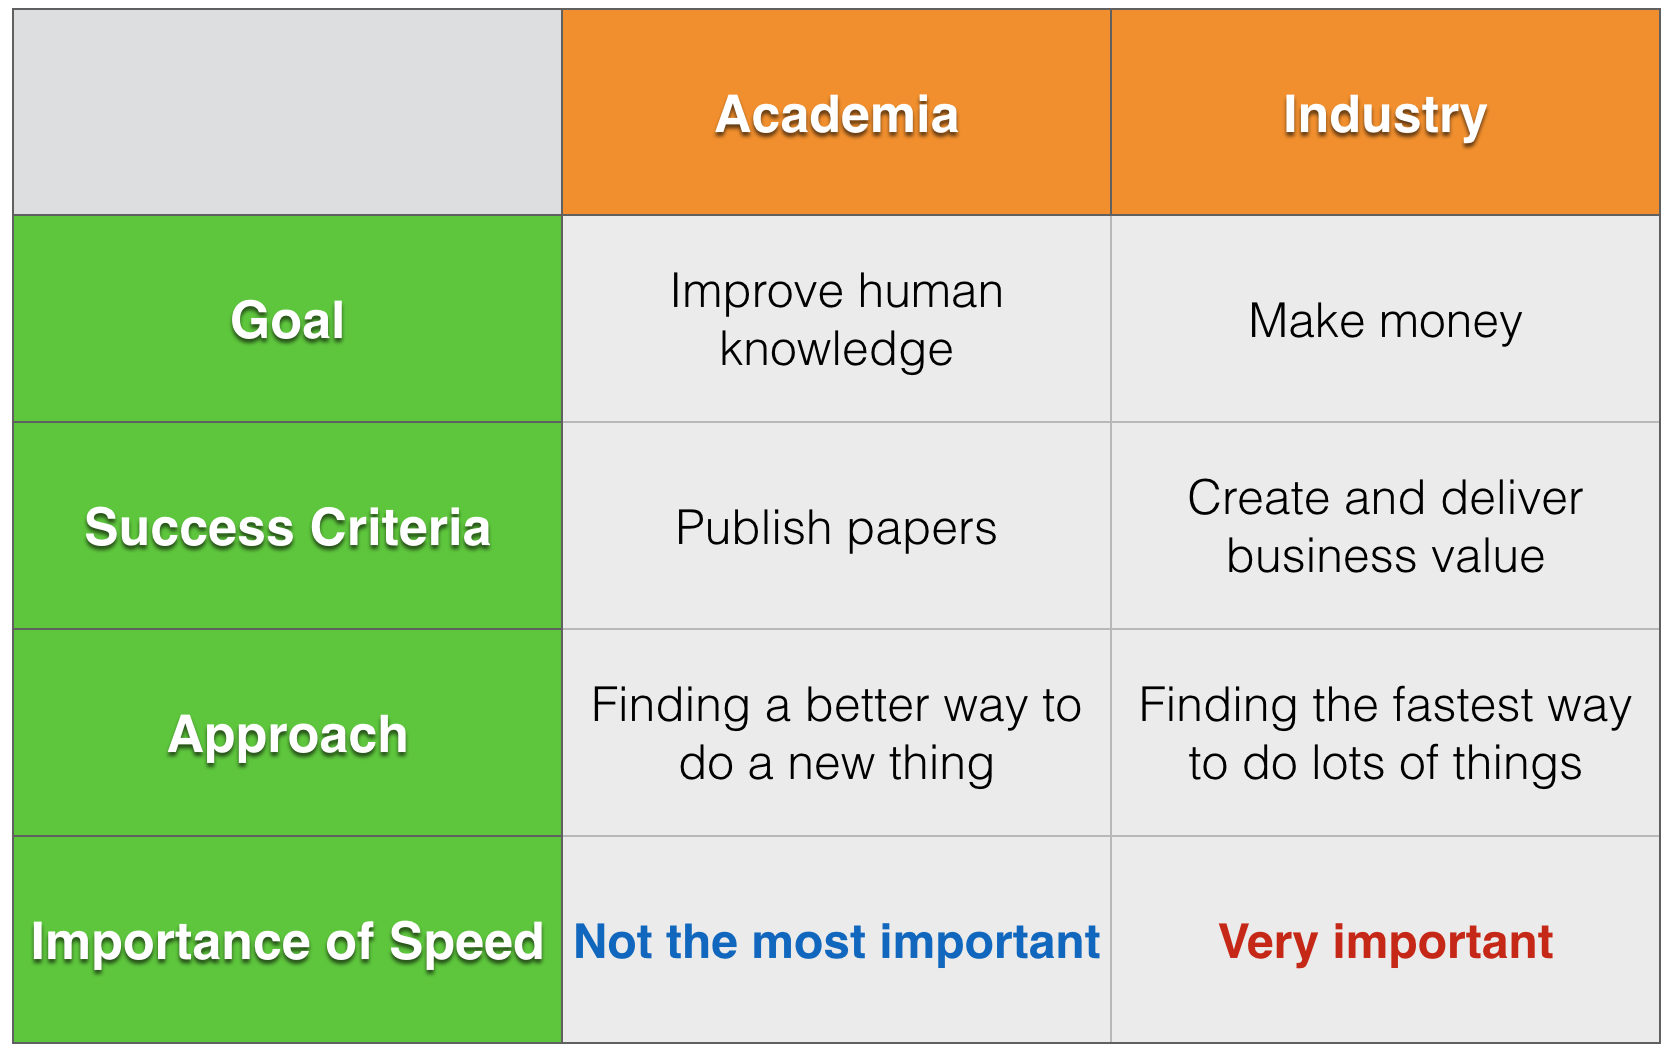
\includegraphics[width=300pt]{../graphs/academia_industry}
      \end{center}
    \end{frame}

    \begin{frame}{Why do we need a toolbox?}
      \begin{center}
        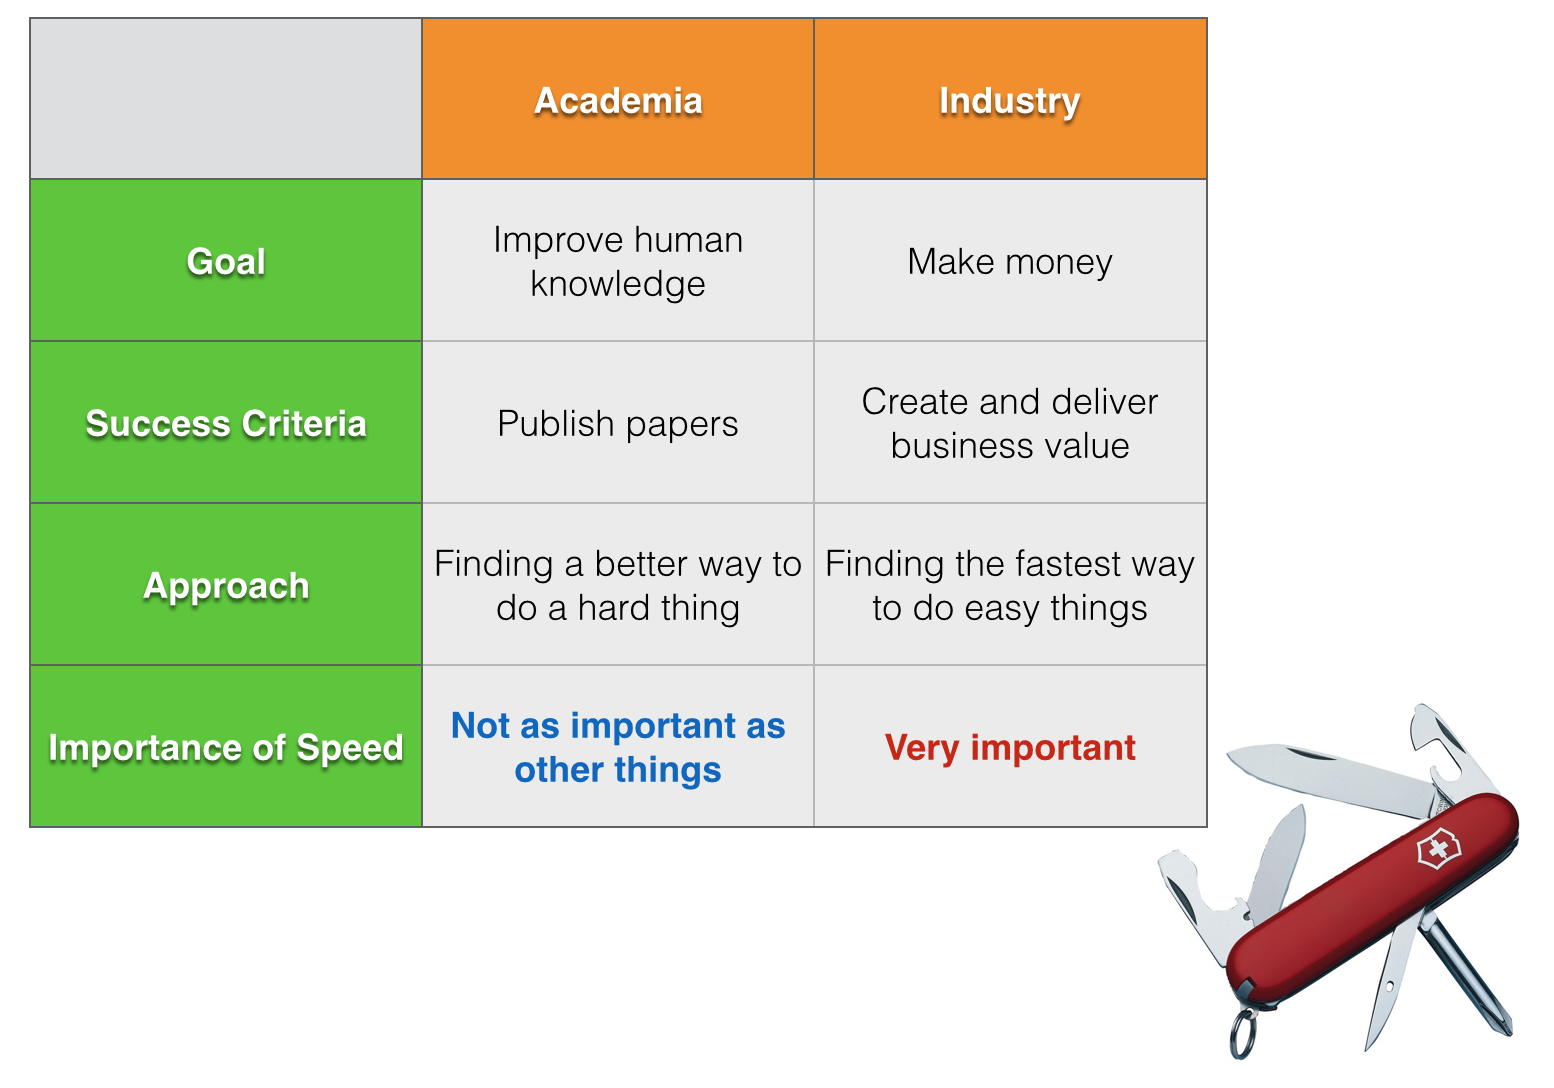
\includegraphics[width=280pt]{../graphs/industry_swiss_army_knife}
      \end{center}
    \end{frame}
    
    \begin{frame}{Python and R for data science}
      \begin{center}
        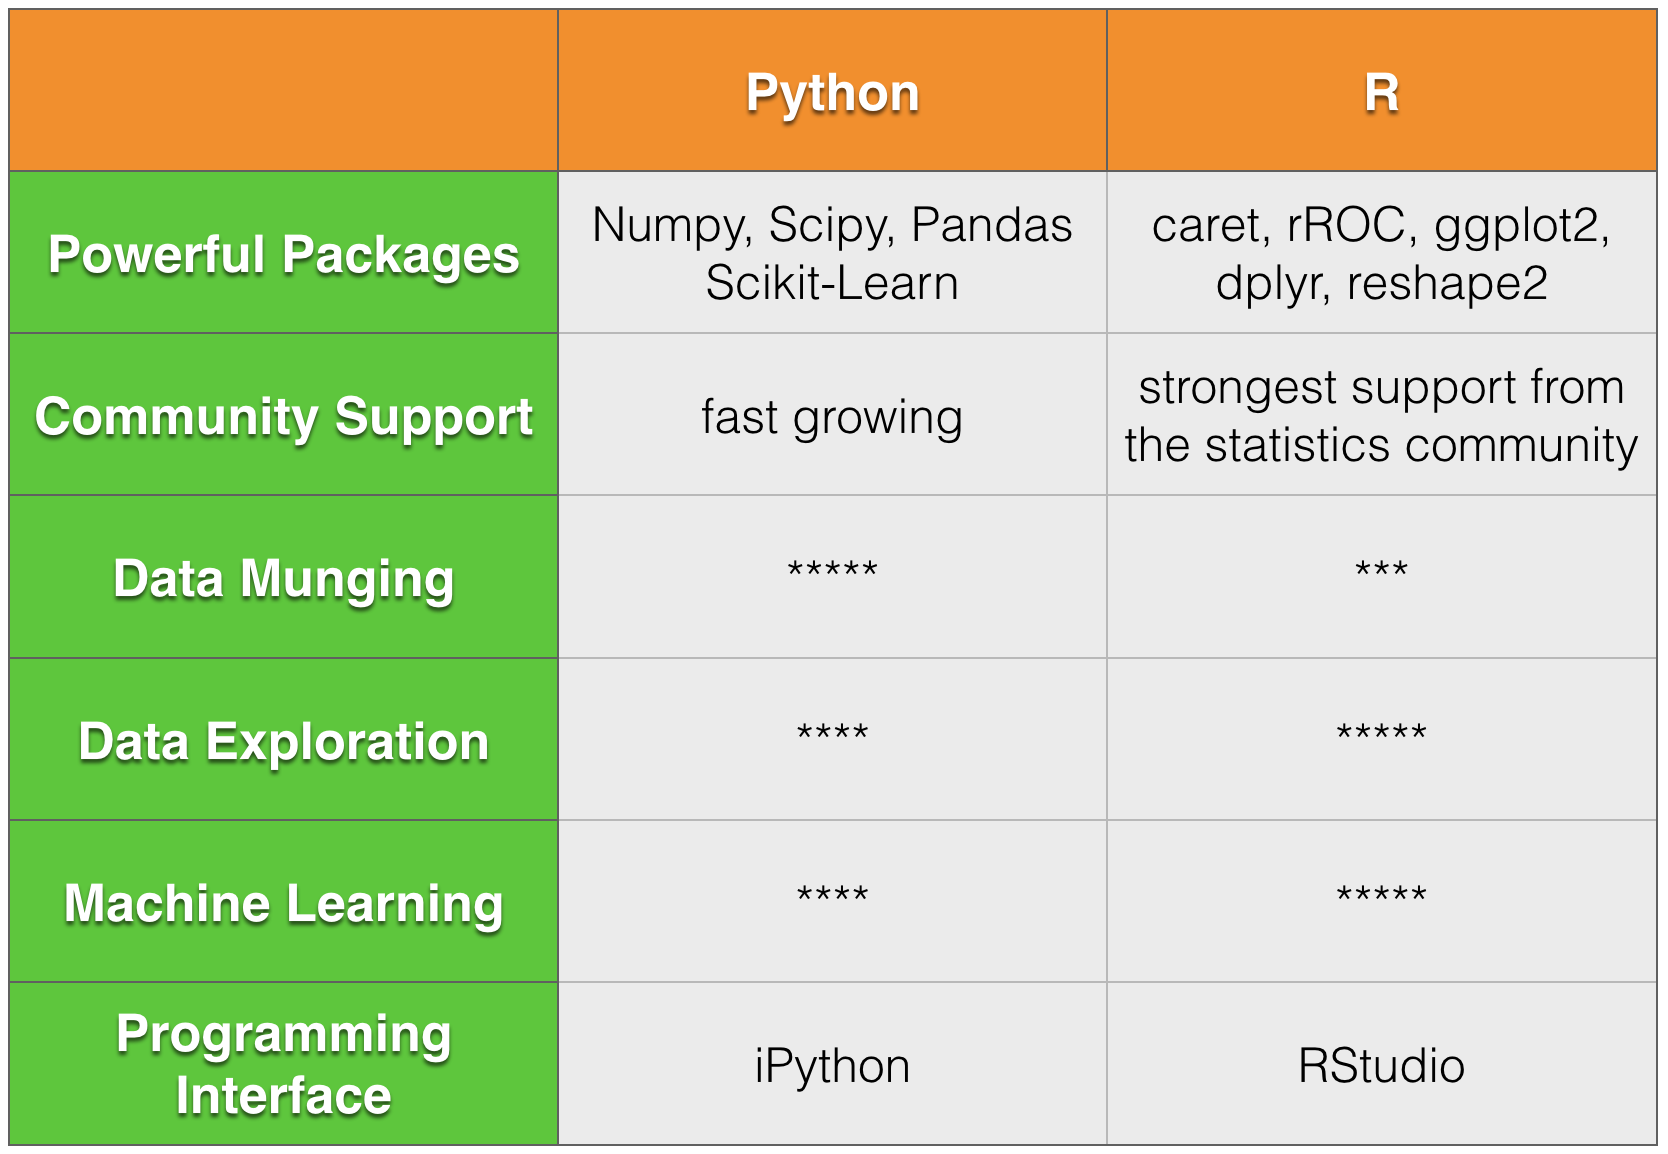
\includegraphics[width=250pt]{../graphs/python_r}
      \end{center}
      {\footnotesize
        iPython \url{http://goo.gl/zT4uPE}
        --- 
        RStudio \url{http://www.rstudio.com/}
      }
    \end{frame}

    \begin{frame}{Data manipulation tools}
      \begin{center}
         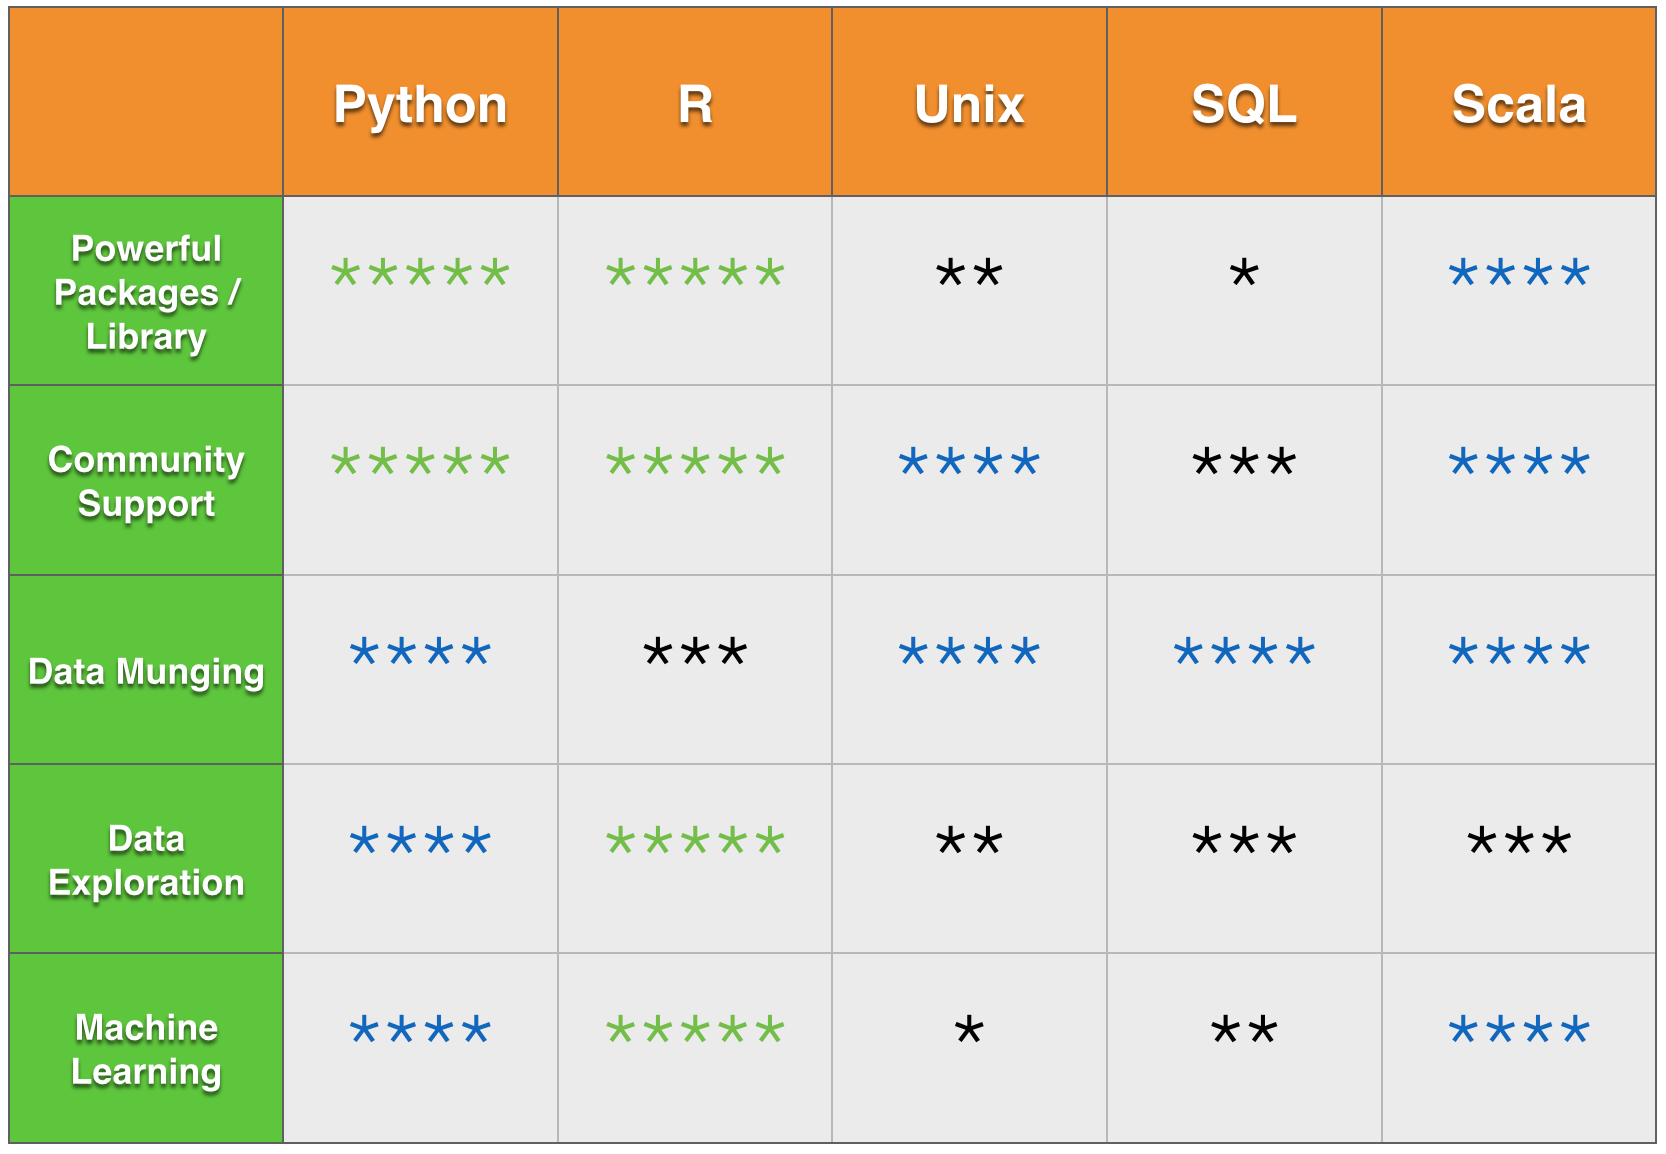
\includegraphics[width=250pt]{../graphs/data_tools}
      \end{center}
    \end{frame}

    \begin{frame}{Data visualization tools}
      \begin{center}
         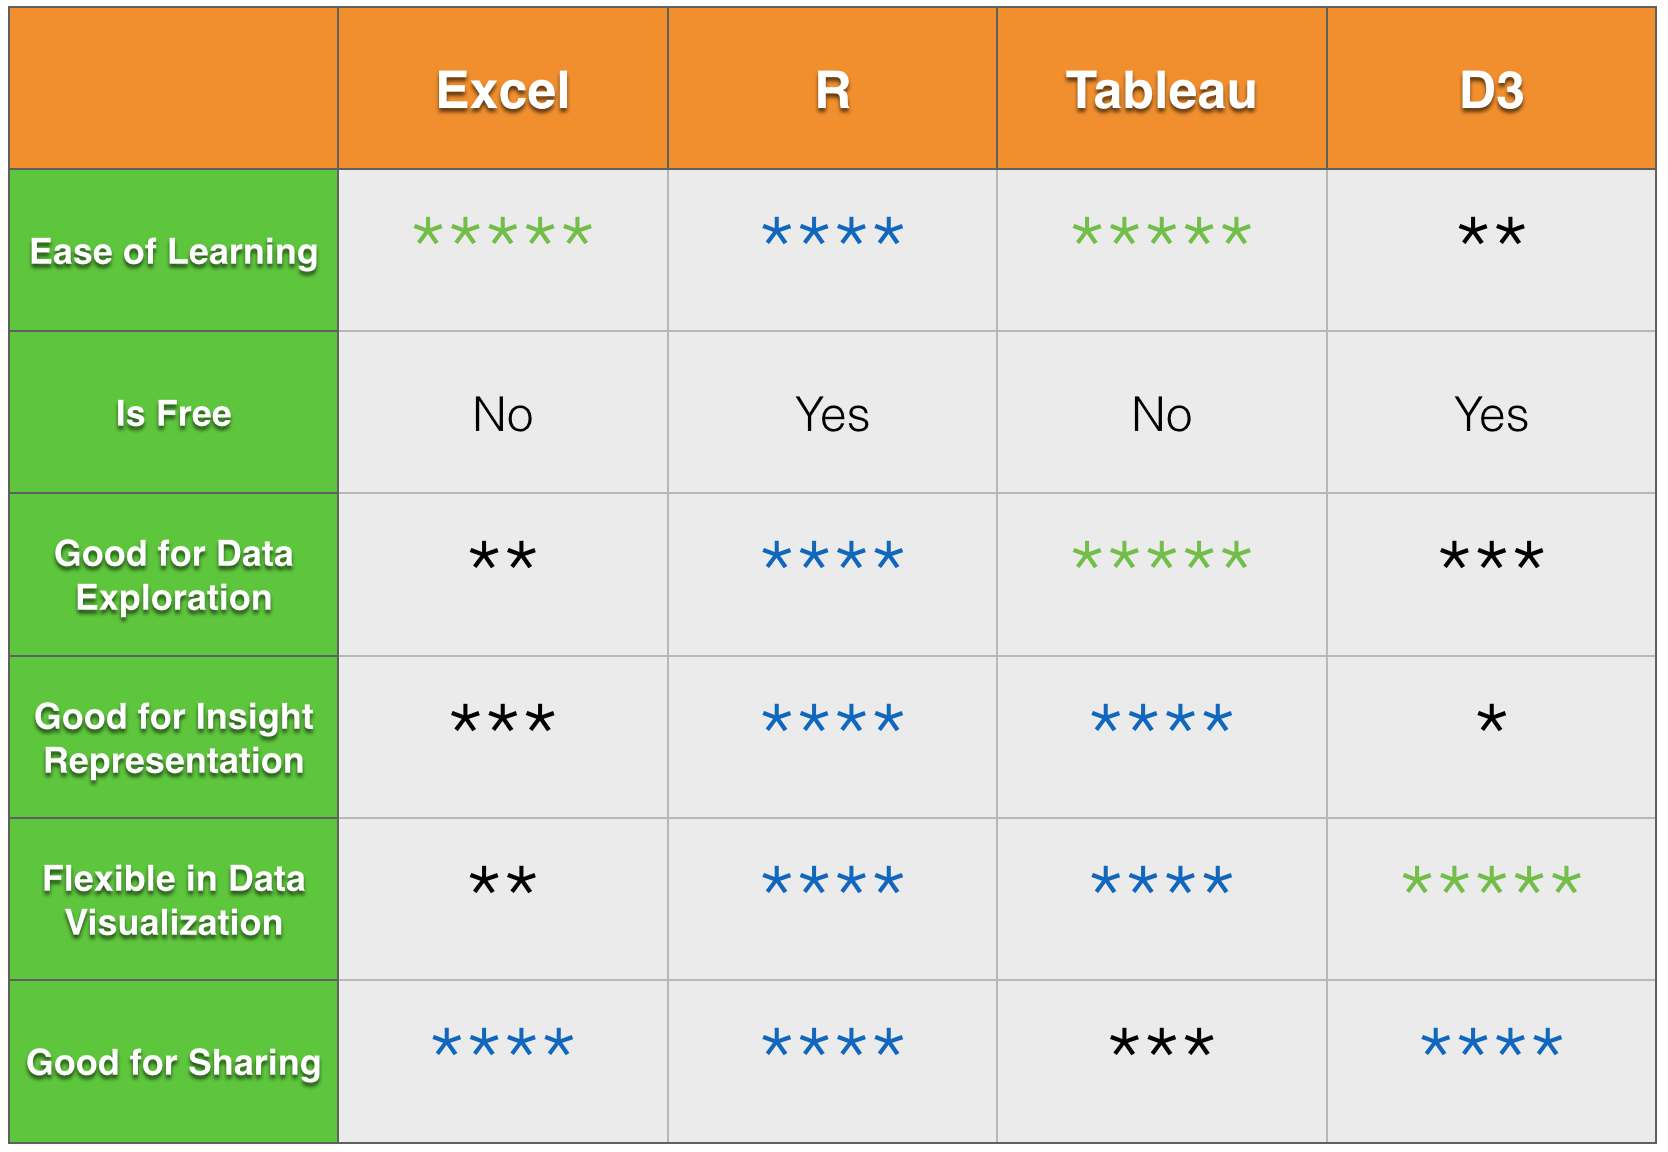
\includegraphics[width=250pt]{../graphs/data_visualization_tools}
      \end{center}
      {\footnotesize
        D3 \url{http://d3js.org/}
      }
    \end{frame}
     
    \begin{frame}{Thank You}
      \centerline{\large Please send your questions and feedbacks to me!}
    \end{frame}

\end{document}